\documentclass{article}
%%%%%%%%% PAPER TYPE  - PLEASE UPDATE FOR FINAL VERSION
%\usepackage[utf8]{inputenc} % allow utf-8 input
\usepackage[T1]{fontenc}    % use 8-bit T1 fonts

% Define conditions
\newif\ifnonanonymous
\newif\ifuseappendix
\newif\ifuseacknowledgement


% ====================
% CONDITIONAL SETTINGS
% ====================
\nonanonymoustrue % comment out to be anonymous
\useacknowledgementtrue % comment out to remove acknowledgements
\useappendixtrue % comment out to remove appendix
% ====================

\ifnonanonymous
\usepackage[nonatbib,final]{neurips_2025}
% to compile a preprint version, e.g., for submission to arXiv, add add the
% [preprint] option:
%     \usepackage[preprint]{neurips_2025}
\else
%\usepackage{neurips_2025}
\usepackage[nonatbib,preprint]{neurips_2025}
\fi

\newcommand{\redact}[1]{%
    \ifnonanonymous
        #1% Show the original text if nonanonymous is true
    \else
        [redacted for peer review]% Redact if false
    \fi
}

% It is strongly recommended to use hyperref, especially for the review version.
% hyperref with option pagebackref eases the reviewers' job.
% Please disable hyperref *only* if you encounter grave issues, 
% e.g. with the file validation for the camera-ready version.
%
% If you comment hyperref and then uncomment it, you should delete *.aux before re-running LaTeX.
% (Or just hit 'q' on the first LaTeX run, let it finish, and you should be clear).
%\definecolor{cvprblue}{rgb}{0.21,0.49,0.74}
%\usepackage[pagebackref,breaklinks,colorlinks,allcolors=cvprblue]{hyperref}
\usepackage{hyperref}


% Include other packages here, before hyperref.
%\usepackage{stfloats}

\usepackage{graphicx}
%\usepackage{emoji}
\usepackage{amsmath}
\usepackage{amssymb}
\usepackage{framed}
\usepackage{booktabs}
\usepackage{comment}
\usepackage{multicol}
\usepackage{makecell}
\usepackage{wrapfig}
\usepackage{subcaption}
\usepackage{cclicenses}


\usepackage{url}            % simple URL typesetting
\usepackage{amsfonts}       % blackboard math symbols
\usepackage{nicefrac}       % compact symbols for 1/2, etc.
\usepackage{microtype}      % microtypography
\usepackage{lipsum}         % Can be removed after putting your text content
\usepackage[numbers]{natbib}
\usepackage{doi}
\usepackage{seqsplit}


%% extra
\usepackage{listings}
\usepackage{amsmath} 
\usepackage{xcolor}
\usepackage[toc]{appendix}

%\usepackage{fontspec}
%\setmainfont{TeX Gyre Termes} % Or another font you like

% Support for easy cross-referencing
\usepackage[capitalize]{cleveref}
\crefname{section}{Sec.}{Secs.}
\Crefname{section}{Section}{Sections}
\Crefname{table}{Table}{Tables}
\crefname{table}{Tab.}{Tabs.}

\newcommand{\cotwo}{\ensuremath{\mathrm{CO_2}}}


\title{``ScatSpotter'' --- A Dog Poop Detection Dataset}

\author{Jonathan Crall\\
Kitware\\
\texttt{jon.crall@kitware.com} \\
%{\tt\small erotemic@gmail.com}
% For a paper whose authors are all at the same institution,
% omit the following lines up until the closing ``}''.
% Additional authors and addresses can be added with ``\and'',
% just like the second author.
% To save space, use either the email address or home page, not both
%\and
%Second Author\\
%Institution2\\
%First line of institution2 address\\
%{\tt\small secondauthor@i2.org}
}

\begin{document}
\maketitle


%%%%%%%%% ABSTRACT
\begin{abstract}


We introduce a new dataset containing phone images of dog feces, annotated with manually drawn or AI-assisted polygon labels.  Its over 9000 ``before/after/negative'' full resolution images contain 6000 polygon annotations.  The collection and annotation of images started in late 2020.  This paper focuses on two checkpoints from 2025-04-20 and 2024-07-03.  We train VIT and MaskRCNN baseline models to explore the difficulty of the dataset.  The best model achieves a pixelwise average precision of 0.858 on a 691-image validation set and 0.810 on a small independently captured 121-image contributor test set.  Dataset snapshots are available through four different distribution methods: two centralized (Girder and HuggingFace) and two decentralized (IPFS and BitTorrent).  We study of the trade-offs between distribution methods and discuss the feasibility of each with respect to reliably sharing open scientific data.  The code for experiments is hosted on GitHub.  The data license is CC-BY 4.0.  Model weights are available with the dataset.  Experiment hardware, time, energy, and emissions are quantified.

% Keywords: poop, feces, dataset, dataset distribution, detection, segmentation, IPFS, BitTorrent, HuggingFace

%We train a baseline vision transformer to segment the objects of interest, exploring a grid of hyperparameters, and we evaluate their impact. 
%A phone application to detect poop with these models is being developed and 
%will be made freely available.
\end{abstract}

%%%%%%%%% BODY TEXT
\section{Introduction}
\label{sec:intro}

Applications for a computer vision system capable of detecting and localizing poop in images are numerous.
These include automated waste disposal to keep parks and backyards clean, tools for monitoring wildlife
  populations via droppings, and a warning system in smart-glasses to prevent people from stepping in poop.
Our primary motivating use case is a phone application that assists dog owners in locating their dog's poop
  in a leafy park for easier cleanup.
Many of these applications can be realized with modern object detection and segmentation methods
  \cite{sandler_mobilenetv2_2018, siam_rtseg_2018, yu_mobilenet_yolo_2023} combined with a large labeled
  dataset. 
%In this paper, we make a significant step towards building this dataset.


\begin{figure}[t]
\centering
\begin{subfigure}[t]{0.49\textwidth}
    \centering
    \includegraphics[width=\linewidth]{figures/zoom_leaf.jpg}
    \caption[]{
        A zoomed in example of an annotated object in a challenging
        condition: a scene cluttered with leaves. The similarity between the leaves
        and the poop causes a camouflage effect that can make detecting it difficult.
        The poop is highlighted in blue.
    }
    \label{fig:HardCase}
\end{subfigure}
\hfill
\begin{subfigure}[t]{0.49\textwidth}
    \centering
    \includegraphics[width=\linewidth]{figures/viz_three_images.jpg}
    \caption[]{
        The ``before/after/negative'' protocol.
        The orange box highlights the location of the poop 
        in the ``before'' image.
        In the ``after'' image, it is the same scene but the poop has been removed.
        The ``negative'' image is a nearby similar scene, potentially with a distractor.
        Note that the object is small relative to the image size.
    }
    \label{fig:ThreeImages}
\end{subfigure}
\caption{(a) A challenging annotation case due to camouflage. (b) The BAN protocol.}
\label{fig:Combined}
\end{figure}
  

\begin{table*}[t]
\caption{Related datasets.
%
Columns list dataset name, number of categories, images, and annotations.
Image W \times{} H gives median image dimensions;
Ann Area$^{0.5}$ is the median square root of annotation area (pixels);
Size is disk requirements in GB; 
Annot Type is the labeling method.
\Cref{fig:compare_allannots} shows the distribution of annotation shapes, sizes, and locations.
%Citations: ImageNet \cite{ILSVRC15}
%MSCOCO \cite{lin_microsoft_2014},
%CityScapes \cite{cordts2015cityscapes},
%ZeroWaste \cite{bashkirova_zerowaste_2022},
%TrashCanV1 \cite{hong2020trashcansemanticallysegmenteddatasetvisual},
%UAVVaste \cite{rs13050965},
%SpotGarbage-GINI \cite{mittal2016spotgarbage},
%TACO \cite{proenca_taco_2020},
%MSHIT \cite{mshit_2020}.
%Of the datasets in this table, ours has the highest image resolution.
%and the smallest annotation size relative to that resolution.
%Of the waste related datasets and in terms of number of images, ours is among the largest, and of the poop related datasets, it is the largest.
}
\label{tab:related_datasets}
\begin{tabular}{lrrrcrrl}
\toprule
Name & \#Cats & \#Images & \#Annots & \makecell{Image\\W \times{} H} & \makecell{Annot\\Area$^{0.5}$} & \makecell{Disk\\Size} & \makecell{Annot\\Type} \\
\midrule
ImageNet\cite{ILSVRC15}    & 1,000 & 594,546 & 695,776 & 500 \times{} 374 & 239 & 166GB & box \\
MSCOCO\cite{lin_microsoft_2014}      & 80 & 123,287 & 896,782 & 428 \times{} 640 & 57 & 50GB & polygon \\
CityScapes\cite{cordts2015cityscapes}  & 40 & 5,000 & 287,465 & 2,048 \times{} 1,024 & 50 & 78GB & polygon \\
ZeroWaste \cite{bashkirova_zerowaste_2022}   & 4 & 4,503 & 26,766 & 1,920 \times{} 1,080 & 200 & 10GB & polygon \\
TrashCanV1\cite{hong2020trashcansemanticallysegmenteddatasetvisual}  & 22 & 7,212 & 12,128 & 480 \times{} 270 & 54 & 0.61GB & polygon \\
UAVVaste\cite{rs13050965}    & 1 & 772 & 3,718 & 3,840 \times{} 2,160 & 55 & 2.9GB & polygon \\
SpotGarbage\cite{mittal2016spotgarbage} & 1 & 2,512 & 337 & 754 \times{} 754 & 355 & 1.5GB & category \\
TACO\cite{proenca_taco_2020}        & 60 & 1,500 & 4,784 & 2,448 \times{} 3,264 & 119 & 17GB & polygon \\
MSHIT\cite{mshit_2020}       & 2 & 769 & 2,348 & 960 \times{} 540 & 99 & 4GB & box \\
Ours        & 1 & 9,296 & 6,594 & 4,032 \times{} 3,024 & 87 & 60GB & polygon \\
\bottomrule
\end{tabular}
\end{table*}

\begin{figure*}[t]
\centering
\includegraphics[width=1.0\textwidth]{plots/appendix/dataset_compare/combo_all_polygons.png.png}
\caption[]{
    A comparison of all of the annotations for different datasets including ours.
    All polygon annotations drawn in a single plot with $0.8$ opacity to
    demonstrate the distribution in annotation location, shape, and size with
    respect to image coordinates.
}
\label{fig:compare_allannots}
\end{figure*}

\begin{figure*}[t]
\centering
\includegraphics[width=1\textwidth]{figures/umap-v3.jpg}%
\caption[]{
    %Example images from the dataset based on 2D UMAP \cite{mcinnes_umap_2020} clusters over the dataset.
    %Each point in the top image is a 2D-projected image embedding. Each
    %numbered orange dot corresponds to three nearby images, which are drawn in columns on the bottom.
    %Annotation boxes are drawn in blue.
    %An interesting observation is that there is a clear separation into two UMAP blobs represents snowy versus (columns 1 and 2)
    %  non-snowy images (columns 3-13). We verified that this pattern holds beyond the examples explicitly shown here.
    Example images from 2D UMAP clusters \cite{mcinnes_umap_2020}.
    Each point in the top image represents a 2D-projected embedding, with numbered orange dots indicating nearby
      images in the bottom columns.
    Blue annotation boxes are shown.
    A clear separation emerges between snowy (columns 1-2) and non-snowy images (columns 3-13).
    %this pattern verified beyond these examples.
    %a 200 image subset
    %  of the dataset.
    %Each row corresponds to a selection from a 2D UMAP projection shown on the left.
    %The highlighted nodes circled in blue in the cluster visualization in each row correspond to the images
    %  with annotations (drawn in green) shown on the right.
}
\label{fig:umap_dataset_viz}
\end{figure*}


In addition to enabling several applications, poop detection is an interesting benchmark problem.
It is relatively simple, with a narrow focus on a single class, making it suitable for exploring the
  capabilities of object detection models that target a single labeled class.
However, the task includes non-trivial challenges such as resolution issues (e.g., camera quality,
  distance), camouflaging distractors (e.g., leaves, pine cones, sticks, dirt, and mud), occlusion (e.g., bushes, overgrown
  grass), and variation in appearance (e.g., old vs. new, healthy vs. sick).
An example of a challenging case is shown in \Cref{fig:HardCase}.
Investigation into cases where this problem is difficult may provide insight
into how to better train object detection and segmentation networks.

Towards these ends we introduce a new dataset which, 
%for the purpose of this paper we call "ScatSpotter".
%we formally call ``ScatSpotter''.
in formal settings, we call ``ScatSpotter''.
Poops are annotated with polygons making the dataset suitable for training detection and segmentation
  models.
In order to assist with annotation and add variation, we collect images using a ``before/after/negative'' (BAN)
  protocol as shown in \Cref{fig:ThreeImages}.

From this data, we train a segmentation model to classify which pixels in an image contain poop and which do
  not.
Our models show strong performance, but there are notable failure cases indicating this problem is difficult
  even for modern computer vision algorithms. 

To enable others to build on our results, it is essential that the dataset is accessible and hosted
  reliably.
Centralized methods are a typical choice, offering high speeds, but they can be costly for individuals,
  often requiring institutional support or paid hosting services.
They are also prone to outages and lack built-in data validation.
In contrast, decentralized methods allow volunteers to host data and offers built-in validation of data
  integrity.
This motivates us to compare and contrast the decentralized BitTorrent \cite{cohen_incentives_2003}, and
  IPFS \cite{benet_ipfs_2014} protocols as mechanisms for distributing datasets.

% VGG2 face got removed.
% https://github.com/ox-vgg/vgg_face2/issues/52

Our contributions are:
1) A challenging new \textbf{open dataset} of images with polygon annotations.
2) A set of trained \textbf{baseline models}.
3) A \textbf{comparison of dataset distribution} methods.
%4) \textbf{Open code and models}.


%-------------------------------------------------------------------------
\section{Related Work}
\label{sec:relatedwork}

To the best of our knowledge, our dataset is currently the largest publicly available collection of
  annotated dog poop images, but it is not the first.
A dataset of 100 dog poop images was collected and used to train a FasterRCNN model
  \cite{neeraj_madan_dog_2019} but this dataset and model are not publicly available.
The company iRobot has a dataset of annotated indoor poop images used to train Roomba j7+ to avoid
  collisions \cite{roomba_2021}, but as far as we are aware, this is not available.
In terms of available poop detection datasets we are only aware of MSHIT~\cite{mshit_2020} which is much
  smaller, only contains box annotations, and the objects of interest are plastic toy poops.

Compared to benchmark object localization and segmentation datasets~\cite{ILSVRC15,
  lin_microsoft_2014,cordts2015cityscapes} ours is much smaller and focused only on a single category.
However, when compared to litter and trash datasets
  \cite{bashkirova_zerowaste_2022,proenca_taco_2020,hong2020trashcansemanticallysegmenteddatasetvisual,mittal2016spotgarbage,rs13050965}
  ours is among the largest in terms of number of images / annotations, image size, and total dataset size.
ZeroWaste~\cite{bashkirova_zerowaste_2022} uses a ``before/after'' protocol similar to our BAN protocol.
%% https://paperswithcode.com/dataset/tackknnno
We provide an overview of these related datasets in \Cref{tab:related_datasets}.
Among all of these, ours stands out for having the highest resolution images and the smallest objects
  relative to that resolution.
For a review of additional waste related datasets, refer to \cite{agnieszka_waste}.

\Cref{sec:distribution} discusses the logistics and tradeoffs between dataset distribution mechanisms
  with a focus on comparing centralized and decentralized methods.
IPFS~\cite{benet_ipfs_2014} and BitTorrent~\cite{cohen_incentives_2003} are the decentralized 
  mechanisms we evaluate, but others exist such as Secure Scuttlebut \cite{tarr_secure_2019} and Hypercore
  \cite{frazee_dep-0002_nodate}, which we did not test.

% Very good overview and comparison of the protocols
% https://blog.mauve.moe/posts/protocol-comparisons
% https://distributed.press/
% hypercore - https://github.com/tradle/why-hypercore/blob/master/FAQ.md#how-is-hypercore-different-from-ipfs
% git,
% Secure Scuttlebut (SSB)

\section{Dataset}
\label{sec:dataset}

Our first contribution is the creation of a new open dataset which consists of images of dog poop in mostly
  urban, mostly outdoor environments, from mostly a single city.
The data is annotated to support object detection and segmentation tasks.
The majority of the images feature fresh poop from three specific medium sized dogs, but there are
  a significant number of images with poops of unknown age and from unknown dogs.

Despite these biases, the dataset has significant image variations.
To provide a gist, we computed UMAP \cite{mcinnes_umap_2020} image embeddings based on ResNet50
  \cite{he2016deep} descriptors display images corresponding with clusters in this embedding in
  \Cref{fig:umap_dataset_viz}.

More details about the dataset are available in a standardized datasheet
\cite{gebru_datasheets_2021} that covers the motivation, composition,
collection, preprocessing, uses, distribution, and maintenance. This will be
distributed with the data itself, and is provided in supplemental material.

\subsection{Dataset Collection}

A single researcher on dog walks photographed fresh dog poop, mostly their own
dogs, but often others. Distance was sometimes varied for diversity. Most
images were taken following the ``before/after/negative'' (BAN) protocol.  
A BAN triple comprises a ``before'' shot of the poop, an ``after'' shot
post removal, and a ``negative'' shot of a nearby lookalike (e.g., pine cones,
leaves).  We only use them for negative sampling, but they could enable
contrastive triplet losses \cite{schroff_facenet_2015}.

The majority of images follow the BAN protocol, but there are exceptions.
The first six months of data collection only involved the ``before/after'' part of the protocol. 
We began collecting the third negative image after a colleague suggested it.
In some cases, the researcher failed or was unable to take the second or third image.
These exceptions are often programmatically identifiable.
  
We also received 121 contributor images, mostly outside the BAN protocol.
These images are held out and used as our test set.
%These are used only for testing and are \emph{excluded} from the analysis in \Cref{subsec:datastat}.
Due to the small size, our main results also include validation scores.
%The small size of this test set is the reason that our main results include
%validation and test scores.

\subsection{Dataset Annotation}

Images were annotated using labelme \cite{wada_labelmeailabelme_nodate}.
Most annotations were initialized using SAM and a point prompt.
All AI polygons were manually reviewed.
In most cases only small manual adjustments were needed, but there were a significant number of cases where
  SAM did not work well and fully manual annotations were needed.
Regions with shadows seemed to cause SAM the most trouble, but there were other failure cases.
Unfortunately, there is no metadata to indicate which polygons were manually created or done using AI.
However, the number of vertices may be a reasonable proxy to estimate this, as polygons generated by SAM
  tend to have higher fidelity boundaries.
The boundaries of the annotated polygons are illustrated in \Cref{fig:compare_allannots}.

Data collected after 2024-07-03 was annotated with the help of models trained
on prior data. Again, all predictions were manually verified or corrected. In
these later cases, false positive annotations were labeled (e.g. stick, leaf),
but because these categories are not labeled exhaustively, we exclude them from
all analysis in this paper.


\begin{figure}[t]
\centering
\begin{subfigure}[t]{0.48\textwidth}
    \centering
    \includegraphics[width=\textwidth]{figures/images_timeofday_distribution.png}
    \caption{
        The time-of-year vs time-of-day of each image show lighting and seasonal
        variation.  On the x-axis, 0 is January 1st. On the y-axis, 0 is
        midnight.  Color estimates daylight based on location (if available).
        Most images are in the day, but many were taken at night with flash or
        long exposure.
    }
    \label{fig:TimeOfDayDistribution}
\end{subfigure}
\hfill
\begin{subfigure}[t]{0.48\textwidth}
    \centering
    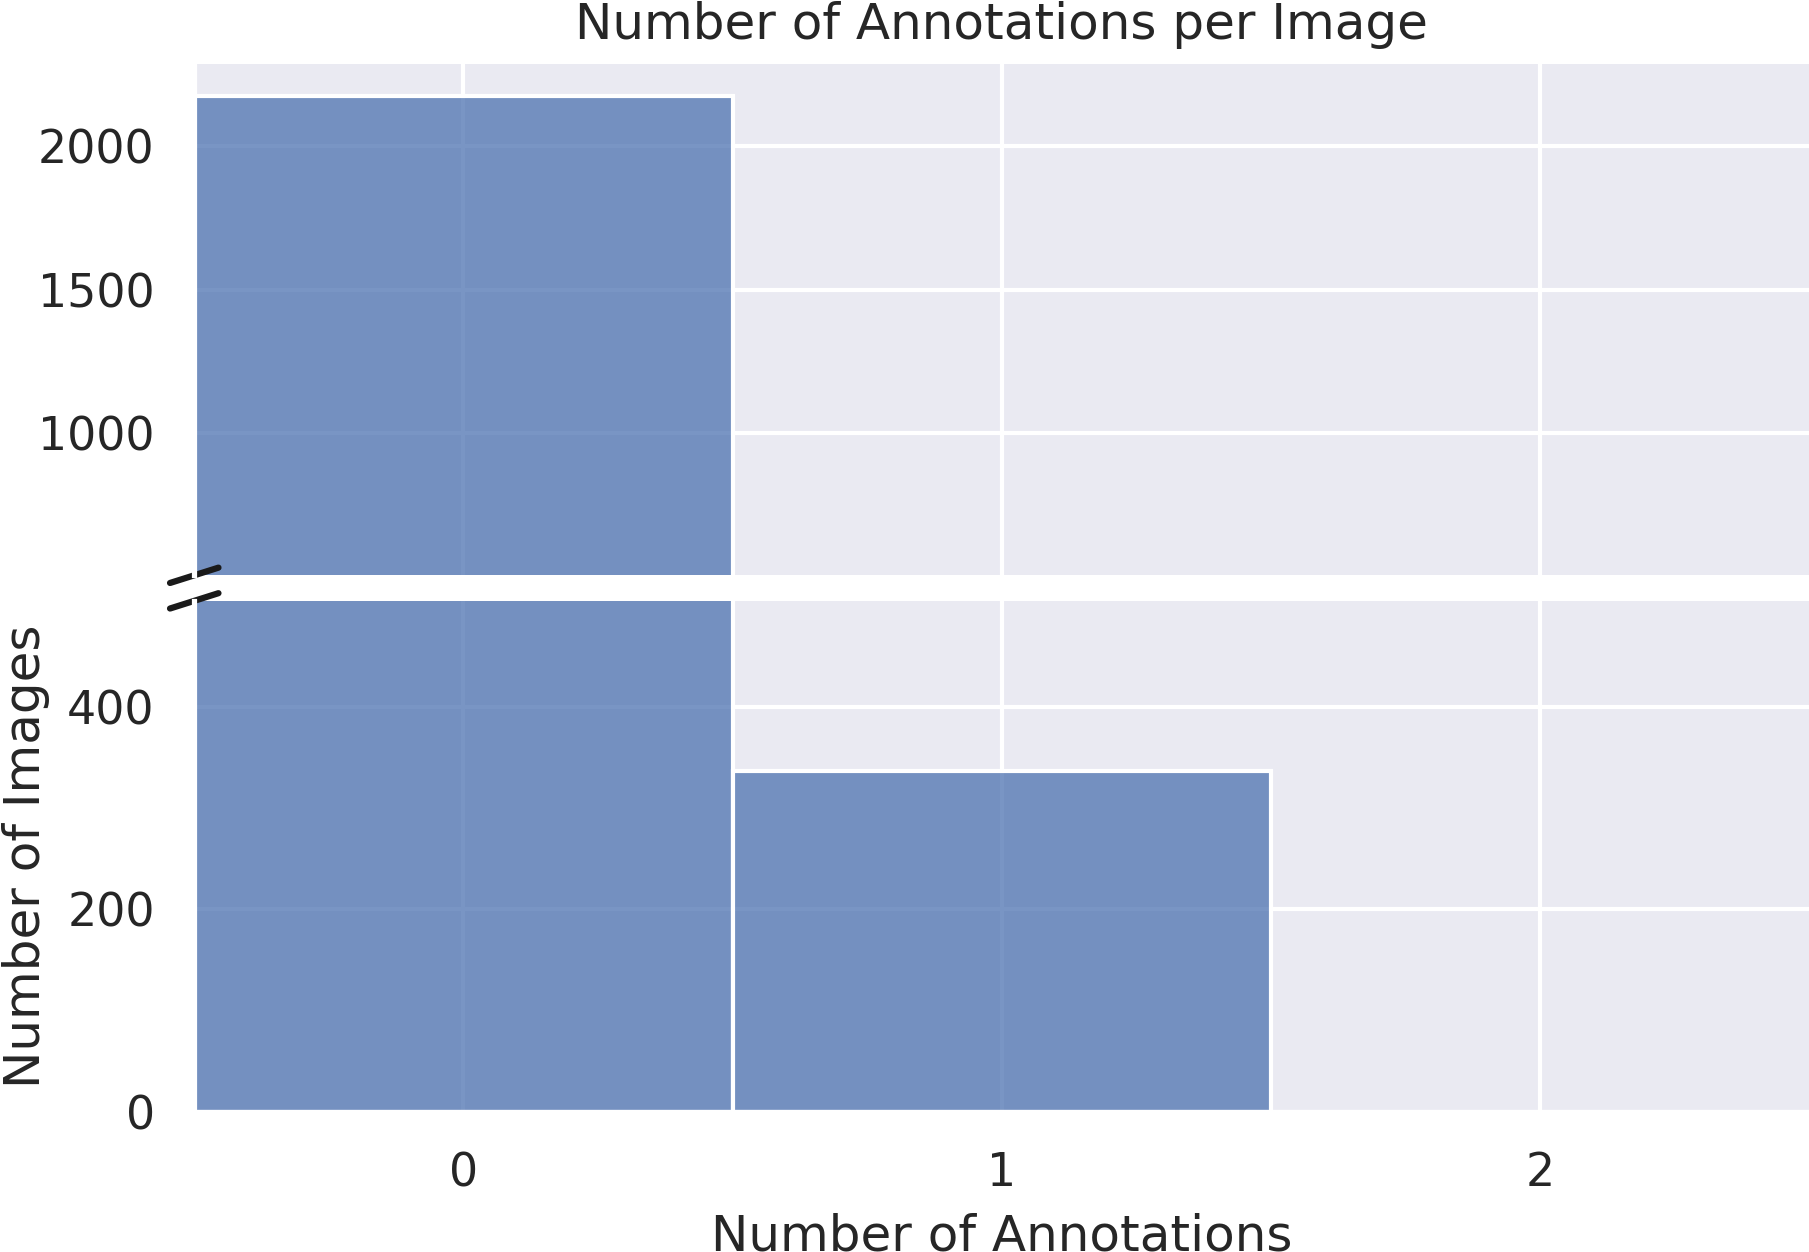
\includegraphics[width=\textwidth]{figures/anns_per_image_histogram_splity.png}
    \caption{
        The histogram of annotations per image shows object density variation.
        Only 35\% (3,314) of images contain annotations; 65\% (5,982) are known negatives.
        About half of the negatives were taken immediately after pickup; the
        rest are from nearby locations with potential lookalikes.
    }
    \label{fig:AnnotsPerImage}
\end{subfigure}
\caption{Dataset distributions. (a) Time and daylight scatterplot. (b) Annotation count histogram.}
\label{fig:TimeAndAnnots}
\end{figure}



\subsection{Dataset Properties and Statistics}
\label{subsec:datastat}

% Number of images, annotations, and other stats.

%import kwutil
%kwutil.datetime.coerce('now') - kwutil.datetime.coerce('2020-12-18')
%kwutil.datetime.coerce('2025-04-20') - kwutil.datetime.coerce('2020-12-18')

The data was captured at a regular rate over 4.3 years, primarily in parks and sidewalks within a small
  city.
Weather conditions varied across snowy, sunny, rainy, and foggy.
A visual representation of the distribution of seasons, time-of-day, daylight, and capture rate is provided
  in \Cref{fig:TimeOfDayDistribution}.

The dataset images are available in full resolution.
Almost all images were taken using the same phone-camera, with a consistent width/height of 4,032
  $\times$ 3,024 (although some may be rotated based on EXIF data).
The images are stored as 8-bit JPEGs with RGB channels, and most include overviews (i.e., image pyramids),
  allowing for fast loading of downscaled versions.
%Six images have a slightly different resolution of 4,008 $\times$ 5,344, and one has a resolution of 7,680
%  $\times$ 1,024.


Due to the BAN protocol, about one-third of the images contain
annotations, the rest were taken after the object(s) were removed.  Consequently, most
images have no annotations. When present, annotations are usually singular, but
multiple annotations are common and can be due to:
1) fragmented dropping,
2) dogs pooping together,
3) repeated poops in the same area over time (sometimes hard to distinguish from dirt).
The number of annotations per image is illustrated in \Cref{fig:AnnotsPerImage}.


\subsection{Dataset Splits}

Our dataset is split into training, validation, and test sets based on the year and day of image capture and
  photographer.
Only data captured by the authors is used for training and validation.
Of these, images from 2021-2023, 2025 and beyond are assigned to the training set. 
Images from 2020 are used for
  validation.
For data from 2024, we consider the ordinal date $n$ of each image and include it in the validation set if
  $n \equiv 0 \ (\textrm{mod}\ 3)$; otherwise, it is assigned to the training set.


For testing data, we use contributor images to not bias our results based on the way the authors took
  images.
These splits are provided in the COCO JSON format \cite{lin_microsoft_2014} as well as a WebDataset
  \cite{huggingfacewebdataset} on HuggingFace.

\section{Baseline Models}
\label{sec:models}

As our second contribution, we trained and evaluated models to establish a baseline for future comparisons.
Specifically we train three model variants.
We trained two MaskRCNN \cite{he2017mask} models (specifically the \texttt{R\_50\_FPN\_3x} configuration),
  one starting from pretrained ImageNet weights (MaskRCNN-p), and one starting from scratch
  (MaskRCNN-s).
We also trained a semantic segmentation vision transformer variant (VIT-sseg-s)
  \cite{Greenwell_2024_WACV,crall_geowatch_2024}, which was only trained from scratch.
Hyperparameters are given in supplemental materials.

For these baseline models, the training data was limited to an older subset taken before 2024-07-03.
Our training dataset consists of 5,747 images and is identified by a suffix of {\tt 1e73d54f}, which is the
  prefix of its content hash.
The validation set contains 691 images and has a suffix of {\tt 99b22ad0}.
The test set, consists of the 121 images, has a suffix of {\tt 6cb3b6ff}, and includes contributor images
  up to 2025-04-20.
The evaluated models were selected based on their validation scores.

We performed two types of evaluations on the models.
``Box'' evaluation computes standard COCO object detection metrics \cite{lin_microsoft_2014}.
MaskRCNN natively outputs scored bounding boxes, but for the VIT-sseg model, we convert heatmaps into boxes
  by thresholding the probability maps and converting taking the extend of the resulting polygons as bounding
  boxes.
The score is taken as the average heatmap response under the polygon.
Bounding box evaluation has the advantage that small and large annotations contribute equally to the score,
  but it can also be misleading for datasets where the notion of an object instance can be ambiguous.

To complement the box evaluation, we performed a pixelwise evaluation, which is more sensitive to the
  details of the segmented masks, but also can be biased towards larger annotations with more pixels.
The corresponding truth and predicted pixels were accumulated into a confusion matrix, allowing us to
  compute standard metrics \cite{powers_evaluation_2011} such as precision, recall, false positive rate, etc.
For the VIT-sseg model, computing this score is straightforward, but for MaskRCNN we accumulate per-box
  heatmaps into a larger full image heatmap, which can then be scored.

Quantitative results for each of these models on box and pixel metrics are shown in
  \Cref{tab:model_results}.
Because the independent test set is only 121 images, we also present results on the larger validation
  dataset.
Corresponding qualitative test results are illustrated in \Cref{fig:test_results_all_models} and validation
  results in \Cref{fig:vali_results_all_models}.

\newcommand{\tb}[1]{\textbf{#1}}

\begin{table}[t]
\caption[]{
    Results for MaskRCNN and VIT models (suffix -p: pretrained, -s: scratch) on test and validation sets.
    Evaluated with box and pixel metrics --- AP (ppv-tpr area) \cite{powers_evaluation_2011} and AUC (tpr-fpr area) --- computed via scikit-learn \cite{scikit-learn}.
    Pretrained models outperform.
    Note: VIT-sseg was tuned more; MaskRCNN may yield better results with similar effort.
    %Results of MaskRCNN and VIT models. A suffix -p is pretrained, and -s is from scratch.
    %Quantitative results on the test and validation datasets.
    %Unsurprisingly, the model starting with pretrained weights scores best.
    %Models are evaluated using bounding-box metrics (under the Box column) as well as pixelwise-segmentation
    %  metrics (under the Pixel column).
    %We consider positive predictive value (ppv or precision), true-positive-rate (tpr or recall), and false positive rate (fpr).
    %The average precision (AP) is the area under the ppv/tpr curve \cite{powers_evaluation_2011}.
    %The AUC is the area under the tpr/fpr curve.
    %Thus AP is more sensitive to ppv and AUC is more sensitive to fpr.
    %All metrics were computed using scikit-learn \cite{scikit-learn}.
    %We note an important limitation of our results:
    %much more time was spent tuning the VIT-sseg model.
    %It is likely that MaskRCNN results could be improved with further tuning.
    %But these are baseline models; our core contribution is the dataset.
}
\label{tab:model_results}
\centering
\begin{tabular}{ll rrrr rrrr}
\toprule
\multicolumn{2}{c}{Dataset split:} & \multicolumn{4}{c}{Test (n=121)} & \multicolumn{4}{c}{Validation (n=691)} \\
%\multicolumn{2}{c}{Evaluation type:} & \multicolumn{2}{c}{Box} & \multicolumn{2}{c}{Pixel} & \multicolumn{2}{c}{Box} & \multicolumn{2}{c}{Pixel} \\
\multicolumn{2}{c}{Evaluation type:} & Box & Box & Pixel & Pixel & Box & Box & Pixel & Pixel \\
%%%                      T-Box        T-Box        T-Pixel      T-Pixel    | V-Box        V-Box        V-Pixel      V-Pixel
Model type & \# Params & AP         & AUC        & AP         & AUC        & AP         & AUC        & AP         & AUC \\
\midrule
MaskRCNN-p & 43.9e6    & \tb{0.613} & \tb{0.697} & \tb{0.810} & 0.849      & \tb{0.612} & \tb{0.721} & \tb{0.858} & 0.905 \\
MaskRCNN-s & 43.9e6    & 0.253      & 0.464      & 0.384      & 0.798      & 0.255      & 0.576      & 0.434      & 0.891 \\
VIT-s      & 25.5e6    & 0.422      & 0.426      & 0.473      & \tb{0.902} & 0.476      & 0.532      & 0.780      & \tb{0.994} \\
\bottomrule
\end{tabular}
\end{table}


\begin{figure*}[t]
\centering
\includegraphics[width=1.0\textwidth]{figures/agg_viz_results/test_imgs30_d8988f8c.kwcoco/results_detectron-pretrained.jpg}%
\hfill
(a) MaskRCNN-pretrained (test set results).
\includegraphics[width=1.0\textwidth]{figures/agg_viz_results/test_imgs30_d8988f8c.kwcoco/results_detectron-scratch.jpg}%
\hfill
(b) MaskRCNN-scratch (test set results).
\includegraphics[width=1.0\textwidth]{figures/agg_viz_results/test_imgs30_d8988f8c.kwcoco/results_geowatch-scratch.jpg}%
\hfill
(c) VIT-sseg-scratch (test set results).
\includegraphics[width=1.0\textwidth]{figures/agg_viz_results/test_imgs30_d8988f8c.kwcoco/results_input_images.jpg}%
\hfill
(d) Input images from the test set.
\caption[]{
    Qualitative results from the top model on the validation set, applied to test images.
    The first three subfigures (a, b, c) display a binarized classification map (true positives in white, false
      positives in red, false negatives in teal, true negatives in black) and the predicted heatmap (before
      binarization).
    Subfigure (d) shows the input image.
    The heatmap binarization threshold was 0.5.
    Failures occur with close-up or deteriorated objects, and camouflage.
    %Qualitative results using the top-performing model on the validation set, applied to a selection of
    %  images from the test set.
    %Subfigure (d) shows the input image for the above predictions.
    %In the first three subfigures (a, b, and c), the top row is a binarized classification map, where true
    %  positive pixels are shown in white, false positives in red, false negatives in teal, and true negatives
    %  in black.
    %The second row in each subfigure is the predicted heatmap, illustrating the model's output before
    %  binarization.
    %The threshold for binarization was set to $0.5$ in all cases.
    %All three methods show clear responses to objects of interest, but cases where objects are close-up 
    %  and partially deteriorated do seem to be a common failure mode.
    %Camouflage is likely a failure case, but this dataset does not contain
    %  many examples.
    
}
\label{fig:test_results_all_models}
\end{figure*}


\begin{figure*}[t]
\centering
\includegraphics[width=1.0\textwidth]{figures/agg_viz_results/vali_imgs691_99b22ad0.kwcoco/results_detectron-pretrained.jpg}%
\hfill
(a) MaskRCNN-pretrained (validation set results).
\includegraphics[width=1.0\textwidth]{figures/agg_viz_results/vali_imgs691_99b22ad0.kwcoco/results_detectron-scratch.jpg}%
\hfill
(b) MaskRCNN-scratch (validation set results).
\includegraphics[width=1.0\textwidth]{figures/agg_viz_results/vali_imgs691_99b22ad0.kwcoco/results_geowatch-scratch.jpg}%
\hfill
(c) VIT-sseg-scratch (validation set results).
\includegraphics[width=1.0\textwidth]{figures/agg_viz_results/vali_imgs691_99b22ad0.kwcoco/results_input_images.jpg}%
\hfill
(d) Inputs from the validation set.
\caption[]{
    %Qualitative results using the top-performing model on the validation set, applied to a selection of
    %  images from the validation set. See \Cref{fig:test_results_all_models} for an explanation of the visualizations.
    %Each model was selected based on its performance on this dataset, which may
    %  cause spurious cases that agree with the truth labels, but this dataset
    %  was never used to compute a gradient, which still make these valuable
    %  results for assessing generalizability. Notably the models were able to
    %  pick out camouflaged cases on the left, but not all on the right.
Qualitative results of the top model on unseen validation images (see \Cref{fig:test_results_all_models} for visualization details). Although never trained on these data, the model's was able to detect camouflaged cases on the left but missed some on the right, indicating generalizability but also room for improvement.}
\label{fig:vali_results_all_models}
\end{figure*}


All models were trained on a single machine with an Intel Core i9-11900K CPU and an NVIDIA GeForce RTX 3090
  GPU.
A key limitation of these results is the imbalance between model types, with 42 out of 44 trained models
  being VIT-ssegs and only two MaskRCNN models, each taking approximately 8 hours to train.
Future work could further optimize MaskRCNN models to improve comparability.
More details on the VIT-sseg experiments can be found in the supplemental materials.

\paragraph{Environmental Impact} The total time spent on prediction and evaluation across all experiments was 15.6 days, with prediction
  consuming 109.63 kWh of energy and causing an estimated emissions of 23.0 \cotwo kg as measured by
  CodeCarbon \cite{lacoste2019codecarbon}.
We estimated train-time resource usage during training using indirect methods, assuming a constant power
  draw of 345W from the RTX 3090 GPU.
Energy consumption was approximated accordingly, while emissions were calculated using a conversion
  ratio of 0.21 $\frac{\textrm{kg}\cotwo{}}{\textrm{kWh}}$ derived from our prediction time measurements.
Based on file timestamps, we estimated that running 44 different training runs took approximately 159.66
  days, resulting in an estimated energy usage and emissions of 1321.99 kWh and 277.612 $\cotwo$ kg,
  respectively.
For context, at $\frac{\$0.16}{\textrm{kWh}}$ and $\frac{\$25.00}{1000 \cotwo \textrm{kg}}$, the cost of training
  and evaluating was $\$229.06$.

\begin{comment}
import pint
reg = pint.UnitRegistry()
reg.define('CO2 = []')
reg.define('dollar = []')
kwh = reg.Unit('kilowatt/hour')
energy_cost = 0.16 * reg.dollar / (kwh)
emission_cost = 25 * reg.dollar / (1000 * reg.CO2 * reg.metric_ton)
energy = 1321.99 * kwh
emission = 277.612 * reg.CO2 * reg.kg
train = (energy * energy_cost + emission * emission_cost)

energy = 109.63 * kwh
emission = 23 * reg.CO2 * reg.kg
eval = (energy * energy_cost + emission * emission_cost)

train + eval
\end{comment}
  

%train$^{*}$ & time        & 158.95 days      &     3.78 days  &   42 \\
%train$^{*}$ & energy      & 1,316.07 kWh     &     31.34 kWh  &   42 \\
%train$^{*}$ & emissions   & 276.37 \cotwo kg & 6.58 \cotwo kg &   42 \\

%todo: train time resource usage for maskrcnn and vit, reacnknowledge
%limitation, break down results over each.

%Report training time, energy usage, and carbon footprint with details in supplemental materials.

\section{Open Data Distribution}
\label{sec:distribution}

%In our context we are mainly concerned with making the data available.
%In other words, given a content identifier, how long does it take to programmatically access the data?
  
%For a comparison of IPFS and BitTorrent on the protocol level see \cite{zebedee_comparing_2023}.
%Another candidate system is a newer similar tool called IPFS (InterPlanetary File System)
%  \cite{benet_ipfs_2014, bieri_overview_2021}.
%To quote the authors:
%"IPFS could be seen as a single BitTorrent swarm, exchanging objects within one Git repository".
%All data down to the block level is content addressable and stored in a Merkle DAG, which can simplify data
%  versioning compared to using a torrent.


%The challenge lies in the fact that designing and documenting an experiment
%sufficiently for reproducibility requires substantial effort and is prone to
%error. We suggest that reducing the friction in accessing the necessary data
%could improve these success rates. Specifically, this involves codifying data
%download and preparation processes. Datasets that are available via decentralized
%and content-addressable are particularly advantageous, as they can guarantee
%the integrity of the data prevent the issue of dead URLs.

%Centralized data distribution has many advantages. It is fast and has low
%traffic overhead. However, it is prone to failure.  
%Cloud storage for a modest amount of data can be expensive.

%In contrast, Decentralized methods can allow information to persist so long as
%at least 1 person has the data.

%However, there are certain drawbacks of decentralized dataset distribution to
%consider. One significant limitation is the potentially substantial connection
%time required to link with peers, particularly when the data lacks a sufficient
%number of "seeders". Furthermore there needs to be a mechanism to connect to
%peers that can share the data.


%For our purposes we 

%%IPFS vs BitTorrent:
%For a comparison of IPFS and BitTorrent on the protocol level see
%\cite{zebedee_comparing_2023}. In our context we are mainly concerned with
%making the data available.

%the main metric we care about is how easy 

%Both IPFS and BitTorrent are both effectively
%content addressable at the dataset level, which makes them both appropriate for our use case.

%We
%care about accessing the data quickly in order to use it.  Thus, our comparison
%is going to focus on download-time measurements.
%Both of which have the ability to use the Kademlia - distributed hash table (DHT) \cite{maymounkov_kademlia_2002}.
%IPFS always uses its DHT, where as BitTorrent the Kademlia-based Mainline
%Tracker can be disabled in favor of 3rd party trackers.
% Overview and comparison of protocols via github gist:
% https://gist.github.com/liamzebedee/224494052fb6037d07a4293ceca9d6e7
% https://gist.github.com/liamzebedee/4be7d3a551c6cddb24a279c4621db74c
%[Steiner, En-Najjary, Biersack 2022]
% See Also:
% Long Term Study of Peer Behavior in the KAD DHT
% https://git.gnunet.org/bibliography.git/plain/docs/Long_Term_Study_of_Peer_Behavior_in_the_kad_DHT.pdf
% We have been crawling the entire KAD network once a day for more than a year to track end-users with static
% IP addresses, which allows us to estimate end-user lifetime and the fraction of end-users changing their KAD ID.

%Both BitTorrent (starting with the v2 protocol introduced in 2017 \cite{cohen_bittorrent_2017}) and IPFS have the capability to recognize when two torrents or content identifiers (CIDs) contain the same file. This enables seeders to provide files to downloaders of either torrent or CID, enhancing the availability and redundancy of the data.
%Both BitTorrent (as of 2017 in the v2 protocol \cite{cohen_bittorrent_2017})
%and IPFS can recognize that two torrents/CID include the same file and seeders
%can provide files to downloaders of the other.


%Additionally, storing data in the cloud can become prohibitively expensive,
%even for modest amounts of data. In contrast, decentralized methods allow
%information to persist as long as at least one individual retains the data.

%Discuss distributing the dataset via IPFS versus centralized distribution
%systems.
%Decentralized Method - IPFS and BitTorrent.
%Centralized Method - Girder

% BitTorrent can be vulnerable to MITM:
% https://www.reddit.com/r/technology/comments/1dpinuw/south_korean_telecom_company_attacks_torrent/


Empirical evidence suggests that a substantial proportion of scientific studies have low reproducibility
  rates, which has raised concerns across various disciplines \cite{baker_reproducibility_2016}.
Ideally, scientific research should be independently reproducible.
Despite higher success rates in computer science (up to 60\%) compared to other fields, there is still room for improvement
\cite{NEURIPS2019_c429429b, collberg2016repeatability, desai_what_2024}.
Addressing this issue requires not just better experimental documentation but also more reliable and
  accessible data distribution methods.
Specifically, this involves robustly codifying data download and preparation processes.


Centralized data distribution methods allow for codified data access by storing URLs that point to datasets
  within the code, offering fast and direct access.
However, this approach lacks robustness.
It can fail if the provider goes offline, changes the URL, or stops hosting the data.
Additionally, cloud storage can be expensive, and users must trust that the provider delivers the correct
  data --- a risk that can be mitigated by using checksums to verify data integrity.
  %though this adds an extra
  %step for experiment designers.

In contrast, decentralized methods allow users to access data in the same way, even if the organization
  hosting the data changes.
%offer greater data longevity, accessibility, and integrity.
By leveraging content-addressable storage, where the dataset checksum acts as both the key to locate and
  validate the data, these methods ensure data integrity and nearly eliminate the risk of dead URLs, provided
  that at least one peer retains the data.
While decentralized systems face challenges such as longer connection times, increased network overhead, and
  the need for a robust peer network, their ability to ensure data access via a static address
  motivates our investigation

Specifically, we focus on two prominent candidates:
BitTorrent and IPFS.
BitTorrent \cite{cohen_incentives_2003, cohen_bittorrent_2017} is a well known sharing protocol that
  originally relied on centralized trackers and databases of torrent files to connect peers.
While trackers and torrent files are still prominent, torrents can be published to a distributed hash table
  (DHT) using the Kademlia algorithm \cite{maymounkov_kademlia_2002}.
This makes it an strong candidate for a decentralized distribution mechanism.
On the other hand, IPFS (InterPlanetary File System) \cite{benet_ipfs_2014, bieri_overview_2021} is a newer
  tool directly build directly on a DHT.
IPFS has been likened to ``a single BitTorrent swarm, exchanging objects within one Git repository''.
%All data down to the block level is content addressable and stored in a Merkle DAG, which can simplify data
%  versioning compared to using a torrent.
%However, both IPFS and BitTorrent are effectively content addressable at the dataset level, which makes them
%  both appropriate for our use case where we seek a static address that can be used to robustly access data.
Both IPFS and BitTorrent are content addressable at the dataset level, which makes them both appropriate for
  our use case where we seek a static address that can be used to robustly access data.

It is worth noting that git-based \cite{chacon2014progit} systems like
  HuggingFace~\cite{huggingface_datasets} with large file storage do gain some decentralized
  properties via multiple remotes, but not content identifiers.

For practitioners, key concerns are how quickly and reliably data can be accessed.
By comparing decentralized and centralized mechanisms access times for our dataset, we aim to make
  explicit the tradeoffs between the methods and inform decisions on adopting an approach.

%identify the most effective method for
%  ensuring that scientific datasets remain accessible and reproducible over time, thereby contributing to
%  improved reproducibility in scientific research


\subsection{Dataset Transfer Experiment}

Our third contribution is an experiment that studies transfer rates of decentralized and centralized data
  distribution methods.
For centralized distribution, we use a self-hosted instance of Girder~\cite{girder_2024} and the HuggingFace
  datasets~\cite{huggingface_datasets} platform.
For decentralized clients, we use Transmission~\cite{transmission_2024} (BitTorrent) and
  Kubo~\cite{ipfskubo_2024} (IPFS).
As a baseline, we also measure direct transfers using Rsync~\cite{rsyncprojectrsync_2024}.

For data transfer experiments, we use the 2024-07-03 version of the dataset. 
This is content-addressed with the IPFS CID (content identifier):
\texttt{\seqsplit{bafybeiedwp2zvmdyb2c2axrcl455xfbv2mgdbhgkc3dile4dftiimwth2y}}
%{\tt bafybei edwp2zvmdyb2c 2axrcl455xfbv 2mgdbhgkc3dil e4dftiimwth2y}.
%{\tt bafybeiedwp2zvmdyb2c2axrcl455xfbv2mgdbhgkc3dile4dftiimwth2y}.
%\begin{lstlisting}[basicstyle=\normalsize]
%bafybeiedwp2zvmdyb2c2axrcl455x
%fbv2mgdbhgkc3dile4dftiimwth2y
%\end{lstlisting}
The torrent has a magnet URL of:
\texttt{\seqsplit{magnet:?xt=urn:btih:ee8d2c87a39ea9bfe48bef7eb4ca12eb68852c49}},
%{\tt magnet:?xt=urn:btih:ee8d2c87a39ea9bfe48bef7eb4ca12eb68852c49},
and is tracked on Academic Torrents \cite{academic_torrents_Cohen2014}.
%\begin{lstlisting}[basicstyle=\normalsize]
%\end{lstlisting}

To assess the effectiveness of each mechanism we programmatically download our 42GB dataset and measure the
  time required to complete the transfer.
Each experiment was run five times, machines we controlled were separated by $\sim\!30$ kilometers
  with an average ping time of 48.48 ms.
For each test, we log transfer start and end times along with notes and code (provided in supplemental
  materials).

While our measurements provide a reasonable estimate of for access time for each mechanism, there are
  notable limitations in our methodology.
First, different machines and networks have different upload and download speeds, and network congestion is
  variable.
For decentralized methods, we lack an automated mechanism separate peer-connection time and actual download
  time.
Additionally, Girder and HuggingFace required data to be packed into compressed archives, improving transfer
  efficiency due to fewer file boundaries.
In decentralized cases, we provide granular access to each file in the dataset, which avoids an extra
  unpacking step and enables sharing of the same file between different versions of the datasets and simpler
  updates, but decreases transfer efficiency.
Due to this, we provide both a compressed and uncompressed rsync baseline.
Another confounding factor is that with decentralized mechanisms the number of seeders is not controlled
  for.
Subsets of the data have been hosted on IPFS for years, and portions of the dataset may be provided by
  unknown members of the network.
For BitTorrent, our initial transfers only had one seeder, but during our tests other nodes accessed and
  started to provide the data.

Despite significant testing limitations, our measurements quantify the expected data-access time penalty to
  gain the advantages of decentralized mechanisms.
With these limitations acknowledged, we present the transfer times statistics in \Cref{tab:transfertime}.
Alongside these measurements, several observations are worth noting.
Transferring files using IPFS had significantly delayed peer discovery times, and we were only able to
  connect two machines after manually informing them of each other's peer ID.
For BitTorrent, were unable to use the mainline DHT and fell back to using trackers.
We believe these peer discovery issues are because the dataset has a small number of seeders.
To test this, we downloaded other established datasets via IPFS and BitTorrent and found that the peer
  discovery time was almost immediate, suggesting that this becomes less of an issue as a dataset is shared.
However, the inability to quickly find a nearby peer is a major issue for initial or private dataset
  development.


%%\begin{wraptable}{r}{0.5\textwidth}
%%\small
%\begin{table}[t]
%%\vspace{-1.2em} % optional tweak
%\caption[]{
%Transfer times (in hours) for our 42GB dataset: trials (n), mean (\mu), std (\sigma).
%Each experiment was run 5 times.
%Suffix (-u) means uncompressed, (-c) means compressed.
%Uncompressed transfers provide granular access to individual files, but compressed transfers are faster.
%}
%\label{tab:transfertime}
%\centering
%\setlength{\tabcolsep}{5.35pt} % Reduce horizontal padding
%\begin{tabular}{lrrrr}
%\toprule
%{}           &        \mu &     \sigma &   Min &    Max \\
%Method       &            &            &       &        \\
%\midrule       
%BitTorrent-u &      8.36h &      5.16h & 2.21h & 14.39h \\
%IPFS-u       &     10.68h &      9.54h & 1.80h & 24.62h \\
%Rsync-u      &      4.84h &      1.39h & 3.10h &  6.10h \\
%Girder-c     &      2.85h &      2.31h & 1.05h &  6.24h \\
%HuggingFace-c & \bf{0.14h} &      0.03h & 0.11h &  0.18h \\
%Rsync-c      &      1.10h &      0.03h & 1.07h &  1.13h \\
%\bottomrule
%\end{tabular}
%%\end{wraptable}
%\end{table}


\begin{table}[t]
\caption{
Transfer times (in hours) for our 42GB dataset: trials (n), mean ($\mu$), std ($\sigma$).
Each experiment was run 5 times.
Uncompressed transfers provide granular access to individual files, while compressed transfers are faster.
}
\label{tab:transfertime}
\centering
\setlength{\tabcolsep}{4.5pt} % Adjusted padding for new column
\begin{tabular}{lcrrrr}
\toprule
Method       & Compressed & $\mu$     & $\sigma$ & Min    & Max     \\
\midrule       
BitTorrent   & No         & 8.36h     & 5.16h    & 2.21h  & 14.39h  \\
IPFS         & No         & 10.68h    & 9.54h    & 1.80h  & 24.62h  \\
Rsync        & No         & 4.84h     & 1.39h    & 3.10h  & 6.10h   \\
Girder       & Yes        & 2.85h     & 2.31h    & 1.05h  & 6.24h   \\
HuggingFace  & Yes        & \bf{0.14h}& 0.03h    & 0.11h  & 0.18h   \\
Rsync        & Yes        & 1.10h     & 0.03h    & 1.07h  & 1.13h   \\
\bottomrule
\end{tabular}
\end{table}

% https://huggingface.co/papers/2307.12169
% https://github.com/huggingface/hf_transfer
% https://github.com/huggingface/datasets
% https://arxiv.org/pdf/1804.07617


The HuggingFace results stand out, as they are faster than rsync.
We believe this is due to an optimized client and content delivery networks, utilizing CAKE
  \cite{hoiland2018piece} to minimize buffer bloat \cite{gettys2012bufferbloat}.
However, this speed relies on costly centralized infrastructure.
The expected speed from a more modest centralized service is $\sim\!20\times$ slower.

There is an additional $\sim\!4\times$  slowdown between compressed and uncompressed rsync baselines, which needs to be
  considered when comparing decentralized results.
The minimum time column shows that decentralized methods method can be competitive with rsync, but on
  average decentralized mechanisms are significantly slower and can be stifled by long peer-discovery times.
  
\section{Conclusion}

We have introduced the largest open dataset of high resolution images with polygon
  segmentations of dog poop.
The dataset contains several challenges including amorphous objects, multi-season variation, difficult
  distractors, daytime / nighttime variation.
We have described the dataset collection and annotation process and reported statistics on the dataset.

We provided a recommended train/validation/test split of the dataset, and trained baseline segmentation
  models that perform well, but could likely be improved.
In addition to providing quantitative and qualitative results of the models, we also estimate the resources
  required to perform these training, prediction, and evaluation experiments.

We have published our data and models under a permissive license, and made them available through both
  centralized (Girder and HuggingFace) and decentralized (BitTorrent and IPFS) mechanisms.
Decentralized methods have robustness properties, but suffer from significant network transfer overhead.
HuggingFace has exceptionally fast transfer speeds, and due to its usage of git-lfs has some decentralized
  properties, but lacks content identifiers.
Combining IPFS with a content distribution network may be a path to a best-of-both-worlds system.
%It may be possible to build a best of both worlds protocol and distribution network.


Limitations of our work include:
1) geographic concentration of the dataset,
2) the small size of the independent test set,
3) limited exploration of the better-performing model variant, and
4) uncontrolled network conditions during distribution experiments.
Future work could address these by expanding dataset diversity, training a
broader range of models, and improving decentralized hosting strategies.

Our dataset enables applications such as mobile apps for detecting feces, urban
cleanliness monitoring, and augmented reality collision warnings. We believe
negative impacts are limited and expect respectful use of the dataset.
We envision exciting possibilities for the BAN protocol in computer vision research.
We hope our work will inspire others to consider decentralized content addressable data sharing, fostering
  open collaboration and reproducible experiments.
Furthermore, we encourage the community to track experimental resource usage to better understand and offset
  our experiments' small, but real environmental impact.
Moreover, we aspire for our dataset to enable the creation of poop-aware applications.
Ultimately, our goal is for this research to contribute meaningfully to the advancement of computer vision
  and have a positive impact on society.
  
  
%\ifnonanonymous
\ifuseacknowledgement
\section{Acknowledgements}
We would would like to thank all of the dogs that produced subject matter for the dataset, all of the
contributors for helping to construct a challenging test set, and \redact{Anthony Hoogs} for several suggestions including taking the 
  third negative picture.
This work is dedicated to \redact{Bezoar}, a very weird and very good girl.
%\fi
\fi

%%%%%%%%% REFERENCES
{\small
\bibliographystyle{ieeenat_fullname}
\bibliography{citations}
}


\ifuseappendix
% WARNING: do not forget to delete the supplementary pages from your submission 
\appendix

\section{Dataset}

\subsection{Additional Comparisons}
\label{sec:expanded_relatedwork}

In \Cref{sec:relatedwork} we compared to related work. Here we expand on this
by comparing our analysis plots. Every dataset is converted into the COCO
format and visualized using the same logic. \Cref{fig:compare_allannots}
visualizes the annotations of all datasets. We make similar visualizations 
for other comparable dataset metrics.
\Cref{fig:combo_anns_per_image_histogram_splity} shows the number of annotations per image.
\Cref{fig:combo_image_size_scatter} shows of image sizes in each dataset.
\Cref{fig:combo_obox_size_distribution_logscale} shows the distribution of width and heights of oriented bounding boxes fit to annotation polygons.
\Cref{fig:combo_polygon_area_vs_num_verts_jointplot} shows the area of each polygon versus the number of vertices (which could be used to estimate the likelihood a polygon was generated by AI for our dataset).
\Cref{fig:combo_polygon_centroid_relative_distribution} shows the distribution of centroid positions (relative to the image size).


\begin{figure*}[ht]
\centering
\includegraphics[width=1.0\textwidth]{plots/appendix/dataset_compare/combo_anns_per_image_histogram_splity.png.png}
\caption[]{
    Number of annotations per image in each dataset.
}
\label{fig:combo_anns_per_image_histogram_splity}
\end{figure*}


\begin{figure*}[ht]
\centering
\includegraphics[width=1.0\textwidth]{plots/appendix/dataset_compare/combo_image_size_scatter.png.png}
\caption[]{
    Image size distributions of each dataset. 
    Ours has two primary width/heights.
}
\label{fig:combo_image_size_scatter}
\end{figure*}


\begin{figure*}[ht]
\centering
\includegraphics[width=1.0\textwidth]{plots/appendix/dataset_compare/combo_obox_size_distribution_logscale.png.png}
\caption[]{
    Oriented bounding box size distributions (log10 scale) of each dataset.
}
\label{fig:combo_obox_size_distribution_logscale}
\end{figure*}

\begin{figure*}[ht]
\centering
\includegraphics[width=1.0\textwidth]{plots/appendix/dataset_compare/combo_polygon_area_vs_num_verts_jointplot_logscale.png.png}
\caption[]{
    Polygon area versus number of vertices (log10 scale) for each dataset.
    The polygons with more vertices are more likely to be AI generated.
}
\label{fig:combo_polygon_area_vs_num_verts_jointplot}
\end{figure*}

\begin{figure*}[ht]
\centering
\includegraphics[width=1.0\textwidth]{plots/appendix/dataset_compare/combo_polygon_centroid_relative_distribution.png.png}
\caption[]{
    Polygon centroid relative distribution for each dataset. It is interesting
    to note patterns in this data. For instance, the outline of a street can be
    seen in CityScapes. In Zero Waste you can see the conveyor belt. ImageNet
    is more uniform. Ours is Gaussian distributed. 
}
\label{fig:combo_polygon_centroid_relative_distribution}
\end{figure*}

\FloatBarrier


\subsection{Additional Information}
\label{sec:expanded_dataset}

In \Cref{sec:dataset} we provided an overview of several dataset statistics.
In this appendix we expand on that with additional plots.
The distribution of image pixel intensities is illustrated in \Cref{fig:spectra}.
The distribution of images collected over time is shown in \Cref{fig:images_over_time}.
The distribution of annotation location is shown in \Cref{fig:centroid_location_distri} and sizes is shown
  in \Cref{fig:annot_obox_size_dist} and \Cref{fig:annot_area_verts_distri}.


\begin{figure*}[ht]
\centering
\includegraphics[width=0.9\textwidth]{figures/spectra.png}
\caption[]{
    The ``spectra'' or histogram of the pixel intensities in the dataset. 
    The dataset RGB mean/std is $[117, 124, 100], [61, 59, 63]$. 
    High and low saturated values occur, but are included in the stats.
    This was run on the older 2024-07-03 snapshot.
}
\label{fig:spectra}
\end{figure*}


\begin{figure*}[ht]
\centering
\includegraphics[width=0.9\textwidth]{figures/appendix/images_over_time.png}
\caption[]{
    The number of images collected over time.
}
\label{fig:images_over_time}
\end{figure*}


\begin{figure*}[ht]
\centering
\begin{subfigure}[b]{0.4\textwidth}
 \includegraphics[width=\textwidth]{figures/appendix/polygon_centroid_absolute_distribution.png}
 \caption{Absolute pixel coordinates.}
 \label{fig:centroid_abs}
\end{subfigure}
\hfill
\begin{subfigure}[b]{0.4\textwidth}
 \includegraphics[width=\textwidth]{figures/appendix/polygon_centroid_relative_distribution.png}
 \caption{Relative image coordinates.}
 \label{fig:centroid_rel}
\end{subfigure}
\caption{The distribution of annotation centroids in terms of (a) absolute image coordinates and (b) relative image coordinates. The absolute centroid distribution is bimodal because some images are taken in landscape mode and other in portrait mode.}
\label{fig:centroid_location_distri}
\end{figure*}


\begin{figure*}[ht]
\centering
\begin{subfigure}[b]{0.4\textwidth}
  \includegraphics[width=\textwidth]{figures/appendix/obox_size_distribution_jointplot.png}
  \caption{Linear scale.}
  \label{fig:annot_obox_size_dist_linear}
\end{subfigure}
\hfill
\begin{subfigure}[b]{0.4\textwidth}
  \includegraphics[width=\textwidth]{figures/appendix/obox_size_distribution_logscale.png}
  \caption{Log10 scale.}
  \label{fig:annot_obox_size_dist_log}
\end{subfigure}
\caption{The distribution of annotation sizes as measured by an oriented bounding box fit to each polygon. (a) shows this plot on a linear scale and (b) show this plot on a log scale.}
\label{fig:annot_obox_size_dist}
\end{figure*}


\begin{figure*}[ht]
\centering
\includegraphics[width=1.0\textwidth]{figures/appendix/polygon_area_vs_num_verts_jointplot.png}
\caption[]{
    The distribution of polygon areas versus the number of vertices in the polygon boundary.
    The SAM model tends to produce polygons with a higher number of vertices
    than manually drawn ones.  For smaller polygons there are two peaks in the
    number of vertices histograms likely corresponding to pure-manual versus
    AI-assisted annotations.
}
\label{fig:annot_area_verts_distri}
\end{figure*}

\FloatBarrier


\section{Data Distribution \& Transfer}
\label{sec:distribution}

%Report training time, energy usage, and carbon footprint with details in supplemental materials.
\begin{comment}
import pint
reg = pint.UnitRegistry()
reg.define('CO2 = []')
reg.define('dollar = []')
kwh = reg.Unit('kilowatt/hour')
energy_cost = 0.16 * reg.dollar / (kwh)
emission_cost = 25 * reg.dollar / (1000 * reg.CO2 * reg.metric_ton)
energy = 1321.99 * kwh
emission = 277.612 * reg.CO2 * reg.kg
train = (energy * energy_cost + emission * emission_cost)

energy = 109.63 * kwh
emission = 23 * reg.CO2 * reg.kg
eval = (energy * energy_cost + emission * emission_cost)

train + eval
\end{comment}
  

%train$^{*}$ & time        & 158.95 days      &     3.78 days  &   42 \\
%train$^{*}$ & energy      & 1,316.07 kWh     &     31.34 kWh  &   42 \\
%train$^{*}$ & emissions   & 276.37 \cotwo kg & 6.58 \cotwo kg &   42 \\

%todo: train time resource usage for maskrcnn and vit, reacnknowledge
%limitation, break down results over each.


%In our context we are mainly concerned with making the data available.
%In other words, given a content identifier, how long does it take to programmatically access the data?
  
%For a comparison of IPFS and BitTorrent on the protocol level see \cite{zebedee_comparing_2023}.
%Another candidate system is a newer similar tool called IPFS (InterPlanetary File System)
%  \cite{benet_ipfs_2014, bieri_overview_2021}.
%To quote the authors:
%"IPFS could be seen as a single BitTorrent swarm, exchanging objects within one Git repository".
%All data down to the block level is content addressable and stored in a Merkle DAG, which can simplify data
%  versioning compared to using a torrent.


%The challenge lies in the fact that designing and documenting an experiment
%sufficiently for reproducibility requires substantial effort and is prone to
%error. We suggest that reducing the friction in accessing the necessary data
%could improve these success rates. Specifically, this involves codifying data
%download and preparation processes. Datasets that are available via decentralized
%and content-addressable are particularly advantageous, as they can guarantee
%the integrity of the data prevent the issue of dead URLs.

%Centralized data distribution has many advantages. It is fast and has low
%traffic overhead. However, it is prone to failure.  
%Cloud storage for a modest amount of data can be expensive.

%In contrast, Decentralized methods can allow information to persist so long as
%at least 1 person has the data.

%However, there are certain drawbacks of decentralized dataset distribution to
%consider. One significant limitation is the potentially substantial connection
%time required to link with peers, particularly when the data lacks a sufficient
%number of "seeders". Furthermore there needs to be a mechanism to connect to
%peers that can share the data.


%For our purposes we 

%%IPFS vs BitTorrent:
%For a comparison of IPFS and BitTorrent on the protocol level see
%\cite{zebedee_comparing_2023}. In our context we are mainly concerned with
%making the data available.

%the main metric we care about is how easy 

%Both IPFS and BitTorrent are both effectively
%content addressable at the dataset level, which makes them both appropriate for our use case.

%We
%care about accessing the data quickly in order to use it.  Thus, our comparison
%is going to focus on download-time measurements.
%Both of which have the ability to use the Kademlia - distributed hash table (DHT) \cite{maymounkov_kademlia_2002}.
%IPFS always uses its DHT, where as BitTorrent the Kademlia-based Mainline
%Tracker can be disabled in favor of 3rd party trackers.
% Overview and comparison of protocols via github gist:
% https://gist.github.com/liamzebedee/224494052fb6037d07a4293ceca9d6e7
% https://gist.github.com/liamzebedee/4be7d3a551c6cddb24a279c4621db74c
%[Steiner, En-Najjary, Biersack 2022]
% See Also:
% Long Term Study of Peer Behavior in the KAD DHT
% https://git.gnunet.org/bibliography.git/plain/docs/Long_Term_Study_of_Peer_Behavior_in_the_kad_DHT.pdf
% We have been crawling the entire KAD network once a day for more than a year to track end-users with static
% IP addresses, which allows us to estimate end-user lifetime and the fraction of end-users changing their KAD ID.

%Both BitTorrent (starting with the v2 protocol introduced in 2017 \cite{cohen_bittorrent_2017}) and IPFS have the capability to recognize when two torrents or content identifiers (CIDs) contain the same file. This enables seeders to provide files to downloaders of either torrent or CID, enhancing the availability and redundancy of the data.
%Both BitTorrent (as of 2017 in the v2 protocol \cite{cohen_bittorrent_2017})
%and IPFS can recognize that two torrents/CID include the same file and seeders
%can provide files to downloaders of the other.


%Additionally, storing data in the cloud can become prohibitively expensive,
%even for modest amounts of data. In contrast, decentralized methods allow
%information to persist as long as at least one individual retains the data.

%Discuss distributing the dataset via IPFS versus centralized distribution
%systems.
%Decentralized Method - IPFS and BitTorrent.
%Centralized Method - Girder

% BitTorrent can be vulnerable to MITM:
% https://www.reddit.com/r/technology/comments/1dpinuw/south_korean_telecom_company_attacks_torrent/

In \Cref{sec:dataset_transfer} we briefly presented a brief set of data distribution experiments.
Here, we provide more background detail, motivation, and discussion.

Empirical evidence suggests that a substantial proportion of scientific studies have low reproducibility
  rates, which has raised concerns across various disciplines \cite{baker_reproducibility_2016}.
Ideally, scientific research should be independently reproducible.
Despite higher success rates in computer science (up to 60\%) compared to other fields, there is still room for improvement
\cite{NEURIPS2019_c429429b, collberg2016repeatability, desai_what_2024}.
Addressing this issue requires not just better experimental documentation but also more reliable and
  accessible data distribution methods.
Specifically, this involves robustly codifying data download and preparation processes.


Centralized data distribution methods allow for codified data access by storing URLs that point to datasets
  within the code, offering fast and direct access.
However, this approach lacks robustness.
It can fail if the provider goes offline, changes the URL, or stops hosting the data.
Additionally, cloud storage can be expensive, and users must trust that the provider delivers the correct
  data --- a risk that can be mitigated by using checksums to verify data integrity.
  %though this adds an extra
  %step for experiment designers.

In contrast, decentralized methods allow users to access data in the same way, even if the organization
  hosting the data changes.
%offer greater data longevity, accessibility, and integrity.
By leveraging content-addressable storage, where the dataset checksum acts as both the key to locate and
  validate the data, these methods ensure data integrity and nearly eliminate the risk of dead URLs, provided
  that at least one peer retains the data.
While decentralized systems face challenges such as longer connection times, increased network overhead, and
  the need for a robust peer network, their ability to ensure data access via a static address
  motivates our investigation

Specifically, we focus on two prominent candidates:
BitTorrent and IPFS.
BitTorrent \cite{cohen_incentives_2003, cohen_bittorrent_2017} is a well known sharing protocol that
  originally relied on centralized trackers and databases of torrent files to connect peers.
While trackers and torrent files are still prominent, torrents can be published to a distributed hash table
  (DHT) using the Kademlia algorithm \cite{maymounkov_kademlia_2002}.
This makes it an strong candidate for a decentralized distribution mechanism.
On the other hand, IPFS (InterPlanetary File System) \cite{benet_ipfs_2014, bieri_overview_2021} is a newer
  tool directly build directly on a DHT.
IPFS has been likened to ``a single BitTorrent swarm, exchanging objects within one Git repository''.
%All data down to the block level is content addressable and stored in a Merkle DAG, which can simplify data
%  versioning compared to using a torrent.
%However, both IPFS and BitTorrent are effectively content addressable at the dataset level, which makes them
%  both appropriate for our use case where we seek a static address that can be used to robustly access data.
Both IPFS and BitTorrent are content addressable at the dataset level, which makes them both appropriate for
  our use case where we seek a static address that can be used to robustly access data.

It is worth noting that git-based \cite{chacon2014progit} systems like
  HuggingFace~\cite{huggingface_datasets} with large file storage do gain some decentralized
  properties via multiple remotes, but not content identifiers.

For practitioners, key concerns are how quickly and reliably data can be accessed.
By comparing decentralized and centralized mechanisms access times for our dataset, we aim to make
  explicit the tradeoffs between the methods and inform decisions on adopting an approach.

%identify the most effective method for
%  ensuring that scientific datasets remain accessible and reproducible over time, thereby contributing to
%  improved reproducibility in scientific research


 
\FloatBarrier

\subsection{Data Distribution Discussion}
\label{sec:datset_discuss}

To assess the effectiveness of each mechanism we programmatically download our 42GB dataset and measure the
  time required to complete the transfer.
Each experiment was run five times, machines we controlled were separated by $\sim\!30$ kilometers with an
  average ping time of 48.48 ms.
For each test, we log transfer start and end times along with notes and code (provided in code repo).

While our measurements provide a reasonable estimate of for access time for each mechanism, there are
  notable limitations in our methodology.
First, different machines and networks have different upload and download speeds, and network congestion is
  variable.
For decentralized methods, we lack an automated mechanism separate peer-connection time and actual download
  time.
Additionally, Girder and HuggingFace required data to be packed into compressed archives, improving transfer
  efficiency due to fewer file boundaries.
In decentralized cases, we provide granular access to each file in the dataset, which avoids an extra
  unpacking step and enables sharing of the same file between different versions of the datasets and simpler
  updates, but decreases transfer efficiency.
Due to this, we provide both a compressed and uncompressed rsync baseline.
Another confounding factor is that with decentralized mechanisms the number of seeders is not controlled
  for.
Subsets of the data have been hosted on IPFS for years, and portions of the dataset may be provided by
  unknown members of the network.
For BitTorrent, our initial transfers only had one seeder, but during our tests other nodes accessed and
  started to provide the data.

Despite significant testing limitations, our measurements quantify the expected data-access time penalty to
  gain the advantages of decentralized mechanisms.
With these limitations acknowledged, we present the transfer times statistics in \Cref{tab:transfertime}.
Alongside these measurements, several observations are worth noting.
Transferring files using IPFS had significantly delayed peer discovery times, and we were only able to
  connect two machines after manually informing them of each other's peer ID.
For BitTorrent, were unable to use the mainline DHT and fell back to using trackers.
We believe these peer discovery issues are because the dataset has a small number of seeders.
To test this, we downloaded other established datasets via IPFS and BitTorrent and found that the peer
  discovery time was almost immediate, suggesting that this becomes less of an issue as a dataset is shared.
However, the inability to quickly find a nearby peer is a major issue for initial or private dataset
  development.


\subsection{Dataset Versions}

An advantage of content identifiers is that they are resistant to link rot as long as at least one peer
  hosts the data, and more importantly, they can never resolve to the wrong content.
This makes them highly attractive for scientific reproducibility.
In this work we relied on two main dataset versions, each specified by a stable content-based identifiers:

\paragraph{Version from 2024-07-03}
\begin{itemize}
  \item IPFS CID: \ipfscid{bafybeiedwp2zvmdyb2c2axrcl455xfbv2mgdbhgkc3dile4dftiimwth2y}
  \item BitTorrent: \magnetlink{ee8d2c87a39ea9bfe48bef7eb4ca12eb68852c49}
\end{itemize}

\paragraph{Version from 2025-04-20}
\begin{itemize}
  \item IPFS CID: \ipfscid{bafybeia2uv3ea3aoz27ytiwbyudrjzblfuen47hm6tyfrjt6dgf6iadta4}
  \item BitTorrent: \magnetlink{27a2512ae93298f75544be6d2d629dfb186f86cf}
\end{itemize}
Note: the hash suffix of the magnet URL can be searched on \url{academictorrents.com}.

At the time of writing, the version of the dataset on HuggingFace is the latest, and we use git tags that
  correspond with the date of release and the IPFS CID to help identify dataset versions.
However, unlike the decentralized methods, these are not guaranteed to point to the expected version of the
  dataset.
At the time of writing the HuggingFace URL is:
\url{https://huggingface.co/datasets/\redact{erotemic}/scatspotter} and the Girder URL is:
\url{https://data.\redact{kitware}.com/?#user/598a19658d777f7d33e9c18b/folder/66b6bc7ef87a980650f41f98}.


\section{Model \& Training Details}
\label{sec:experiment_details}

In \Cref{sec:models} we provided our main results.
However, a key limitation of these results is the imbalance between model types, with 42 of 47 trained
  models being VIT-ssegs, 2 MaskRCNN models, 2 YOLO models, and 1 tuned GroundingDino model.
Future work could further optimize MaskRCNN, Grounding~DINO, YOLO, and other models to improve both
  performance and comparability, but these results are enough to establish a useful baseline.

For non-VIT models we adhered as closely as possible to the default parameters of their respective
  frameworks, applying changes needed to support our generalized KWCoco format and to fit on a single GPU.
For complete details, we provide links to the training and evaluation scripts for each model family (see
  below).
A docker image with dependencies pre-installed is also available:
\dockerimage
  {https://hub.docker.com/layers/\redact{erotemic}/shitspotter/latest/images/sha256-aec306e515a5c8bef162c872c96b6a82ff3f4798f4b796f1431ce8f1f6288747}
  {\redact{erotemic}/shitspotter:latest}.

\paragraph{Experiment scripts (by task).}

\begin{itemize}
  \item \textbf{Grounding~DINO:}
    \repolink{experiments/grounding-dino-experiments}{./experiments/grounding-dino-experiments}

  \item \textbf{YOLO-v9:}
    \repolink{experiments/yolo-experiments}{./experiments/yolo-experiments}

  \item \textbf{MaskRCNN:}
    \repolink{experiments/detectron2-experiments}{./experiments/detectron2-experiments}

  \item \textbf{VIT-sseg:}
    \repolink{experiments/geowatch-experiments}{./experiments/geowatch-experiments}
\end{itemize}


\subsection{Grounding Dino}

GroundingDINO was evaluated in two modes.
The zero-shot setting used the \hflink{IDEA-Research/grounding-dino-tiny} model from HuggingFace, applied
  directly to our validation and test splits with a fixed set of 10 prompts.
The tuned variant used the community \ghlink{longzw1997/Open-GroundingDino} implementation, initialized from
  \DINOPretrained{} with a BERT text encoder on a single GPU.
Training data was converted to ODVG JSONL format, and the label set reduced to two classes (``poop'' and
  ``unknown'').

The preprocessing pipeline resized the shorter side of each image to 800 pixels while maintaining aspect
  ratio, corresponding to a median scale factor of $\sim$0.26 for our dataset.

In the zero-shot evaluation, we tested ten prompts and selected ``animalfeces'' based on the highest
  validation Box-AP.
\Cref{tab:prompt_variations} shows the full ablation, illustrating that prompt choice strongly affects
  performance.
Prompt choice has a large effect, and the best prompt differs between validation and test splits, but
  overall zero-shot results remain low.


%Grounding DINO zero-shot prompt ablation:
%In \Cref{sec:models} we performed a zero-shot detection experiment with Grounding Dino. This required us to choose a prompt. We evaluated 10 possible choices on the validation set and chose the one with the highest Box AP. Results each variation is given in \Cref{tab:prompt_variations}.

\begin{table*}[t]
\caption{Zero-shot detection results with varied prompts. The chosen prompt has a significant impact on scores, and the best prompt is different between validation and test datasets, but overall zero-shot results are all low scoring. Because this is a zero-shot setting, the validation set can be compared to the test set. Interestingly, the validation scores significantly lower than the test scores indicating a greater degree of difficulty. }
\label{tab:prompt_variations}
\centering
\begin{tabular}{lllllllll}
\toprule
\multicolumn{1}{l}{} & \multicolumn{4}{c}{Validation (n=691)} & \multicolumn{4}{c}{Test (n=121)} \\
 Prompt      & \makecell{AP\\Box}   & \makecell{AUC\\Box}   & \makecell{F1\\Box}   & \makecell{TPR\\Box}   & \makecell{AP\\Box}   & \makecell{AUC\\Box}   & \makecell{F1\\Box}   & \makecell{TPR\\Box}   \\
\midrule
 stool       & 0.01                 & 0.03                  & 0.07                 & 0.07                  & 0.05                 & 0.08                  & 0.18                 & 0.13                  \\
 droppings   & 0.02                 & 0.10                  & 0.14                 & 0.23                  & 0.08                 & 0.14                  & 0.27                 & 0.30                  \\
 petwaste    & 0.04                 & 0.14                  & 0.15                 & 0.25                  & 0.20                 & 0.25                  & 0.35                 & 0.34                  \\
 poop        & 0.04                 & 0.10                  & 0.17                 & 0.16                  & 0.17                 & 0.18                  & 0.31                 & 0.26                  \\
 dogpoop     & 0.05                 & 0.16                  & 0.17                 & 0.20                  & 0.24                 & 0.28                  & 0.38                 & 0.39                  \\
 caninefeces & 0.05                 & 0.16                  & 0.18                 & 0.29                  & 0.17                 & 0.24                  & 0.37                 & 0.39                  \\
 turd        & 0.05                 & 0.18                  & 0.18                 & 0.22                  & \textbf{0.27}        & \textbf{0.32}         & 0.39                 & 0.35                  \\
 feces       & 0.06                 & 0.21                  & 0.18                 & 0.27                  & 0.16                 & 0.26                  & 0.32                 & 0.39                  \\
 excrement   & 0.07                 & \textbf{0.22}         & 0.20                 & 0.28                  & 0.25                 & 0.31                  & 0.39                 & \textbf{0.42}         \\
 dogfeces    & 0.07                 & 0.21                  & \textbf{0.20}        & \textbf{0.31}         & 0.23                 & 0.29                  & \textbf{0.40}        & 0.38                  \\
 animalfeces & \textbf{0.08}        & 0.21                  & 0.20                 & 0.25                  & 0.23                 & 0.30                  & 0.39                 & 0.38                  \\
\bottomrule
\end{tabular}
\end{table*}


\subsection{YOLO-v9}

YOLO-v9 experiments were based on the community \ghlink{WongKinYiu/yolov9} implementation.
We trained both pretrained (ImageNet-initialized) and from-scratch variants, using our fork adapted for
  KWCoco input.

All images were resized to 640$\times$640, corresponding to a median scale factor of $\sim$0.16.
Training used a batch size of 16 with batch accumulation set to 50, for an effective batch size of 800.
Optimization used AdamW with learning rate $3\times10^{-4}$ and weight decay of 0.01.
The pretrained runs started from \YOLOPretrained{}.


\subsection{MaskRCNN}

MaskRCNN experiments were run using a Detectron2 fork with KWCoco support.
Both pretrained and from-scratch models used the standard \texttt{R\_50\_FPN\_3x.yaml} configuration,
  differing only in initialization:
pretrained models used \MaskRCNNPretrained{}, while the from-scratch models started randomly.

To fit training on a single GPU, we reduced the learning rate to $2.5\times10^{-4}$, set the batch size to
  2, and trained for a maximum of 120{,}000 iterations.
The maximum image dimension was capped at 1024, giving a median downsample factor of $\sim$0.25 for our
  dataset.


\subsection{VIT-sseg}
\label{sec:vit_models}

This subsection provides additional details on VIT-sseg models, which were the first architecture we
  explored for this problem and therefore have the most extensive analysis compared to other networks.

To train VIT-sseg models we use the training, prediction, and evaluation system presented in
  \cite{Greenwell_2024_WACV, crall_geowatch_2024}, which utilizes polygon annotations to train a pixelwise
  binary segmentation model.

In all experiments, we use half-resolution images, which means most images have an effective width $\times$
  height of 2,016 $\times$ 1,512.
We employ a spatial window size of 416 $\times$ 416 for network inputs, which means that multiple windows
  are needed to predict on entire images.
During prediction, we apply a window overlap of 0.3 with feathered stitching to prevent boundary artifacts.

To address the class imbalance in our dataset (where positives are patches containing annotations and
  negatives contain no annotations), we adopt a balanced sampling strategy.
Each ``epoch'' consists of randomly sampling 32,768 patches from the dataset with replacement, ensuring
  roughly equal numbers of positive and negative samples.
We train each network for 163,840 gradient steps.
For data augmentation we use random crops and flips.

Our baseline architecture is a variant \cite{bertasius2021space,Greenwell_2024_WACV} of a vision-transformer
  \cite{dosovitskiy_image_2021}.
The model is a 12-layer encoder backbone with 384 channels and 8 attention heads that feeds into a 4-layer
  MLP segmentation head.
It has 25,543,369 parameters and a size of 114.19 MB on disk.
At predict time it uses 1.96GB of GPU RAM.

We compute loss pixelwise using Focal Loss \cite{ross2017focal} with a small downweighting of pixels towards
  the edge of the window.
Our optimizer is AdamW \cite{loshchilov_decoupled_2018}, and we experiment with varying learning rate,
  weight decay, and perturb-scale (implementing the shrink perturb trick~\cite{ash_warm_starting_2020,dohare_loss_2023}).
We employ a OneCycle learning rate scheduler \cite{smith2019super} with a cosine annealing strategy and
  starting fraction of 0.3.
Our effective batch size is 24 with a real batch size of 2 and 12 accumulate gradient steps.
This setup consumes approximately 20 GB of GPU RAM during training.

\subsubsection{VIT-sseg Model Experiments}

To establish a baseline, we evaluated 35 training runs where we varied input resolutions, window sizes,
  model depth, and other parameters.
Although this initial search was somewhat ad-hoc, it provided insights into the optimal configuration for
  our model.
Building on the best hyperparameters from this search, we performed a sweep over 7 combinations of learning
  rate, weight decay, and perturb scale (i.e., shrink and perturb
  \cite{ash_warm_starting_2020,dohare_loss_2023}).
Scripts used to reproduce these experiments, as well as a log of the ad-hoc experiments, are available in
  the code repository.
Additionally, trained models are packaged and distributed with information about their training
  configuration.

Note:
the test dataset used in this appendix section is an older 30 image version with suffix {\tt d8988f8c},
  which is a subset of the more recent 121 image test set used in the main paper.


\begin{table*}[t]
\caption{
Results for the best-performing models on the validation set across 7 hyperparameter configurations.
The table provides detailed information about each configuration, including:
1) Configuration name (first column): a unique code identifying each training run used in the score scatter and box plots.
2) Varied hyperparameters (next three columns): specific values for learning rate, weight decay, and perturb scale that were used in each run.
3) Validation set performance (AP and AUC scores): metrics evaluating the model's performance on the validation set.
4) Test set performance (AP and AUC scores): metrics evaluating the model's performance on the test set using the same validation-maximizing models.
Note that the top AP score over all models on the test set was 0.65, but it did not correspond to one of these validation runs used for model selection.
Qualitative examples illustrating the performance of the top-scoring validation model listed here are provided in \cref{fig:test_heatmaps_with_best_vali_model}.
}
\label{tab:parameters_and_results}
\centering
\begin{tabular}{llllllll}
\toprule
            \multicolumn{4}{l}{} & \multicolumn{2}{r}{Validation (n=691)} & \multicolumn{2}{r}{Test (n=30)} \\
Config Name  &   LR & Weight Decay & Perterb Scale & \makecell{AP\\Pixel} & \makecell{AUC\\Pixel} &  \makecell{AP\\Pixel} &  \makecell{AUC\\Pixel} \\
\midrule
        \textcolor[HTML]{623682}{D05} & 1e-4 &   1e-6 &  3e-6 & \textbf{0.7802} & \textbf{0.9943} &          0.5051 &          0.9125 \\
        \textcolor[HTML]{df8020}{D03} & 1e-4 &   1e-5 &  3e-7 &          0.7758 &          0.9707 &          0.4346 &          0.8576 \\
        \textcolor[HTML]{87b787}{D04} & 1e-4 &   1e-7 &  3e-7 &          0.7725 &          0.9818 &          0.4652 &          0.7965 \\
        \textcolor[HTML]{207fdf}{D02} & 1e-4 &   1e-6 &  3e-7 &          0.7621 &          0.9893 & \textbf{0.5167} & \textbf{0.9252} \\
        \textcolor[HTML]{20df20}{D00} & 3e-4 &   3e-6 &  9e-7 &          0.7571 &          0.9737 &          0.4210 &          0.7766 \\
        \textcolor[HTML]{df20df}{D01} & 1e-3 &   1e-5 &  3e-6 &          0.7070 &          0.9913 &          0.4607 &          0.9062 \\
        \textcolor[HTML]{b00403}{D06} & 1e-4 &   1e-6 &  3e-8 &          0.6800 &          0.9773 &          0.4137 &          0.8157 \\
        
\bottomrule
\end{tabular}
\end{table*}

\begin{comment}
    SeeAlso:
    ~/code/shitspotter/experiments/geowatch-experiments/run_pixel_eval_on_vali_pipeline.sh
    python ~/code/shitspotter/dev/poc/estimate_train_resources.py
\end{comment}

For each of the 7 hyperparameter combinations, we trained the model for 163,840 optimizer steps using a
  batch size of 24.
We defined an ``epoch'' as 1,365 steps, at which point we saved a checkpoint, evaluated validation loss, and
  adjusted learning rates.
To conserve disk space, we retained only the top 5 lowest-validation-loss checkpoints (although training
  crashes and restarts sometimes resulted in additional checkpoints, which are included in our evaluation).

Using the top-checkpoints, we predicted heatmaps for each image in the validation set.
We then performed binary classification on each pixel (poop-vs-background) using a threshold.
Next, we rasterized the truth polygons.
The corresponding truth and predicted pixels were accumulated into a confusion matrix, allowing us to
  compute standard metrics such as precision, recall, false positive rate, etc.
\cite{powers_evaluation_2011} for the specific threshold.
By sweeping a range of thresholds, we calculated the average precision (AP) and the area under the ROC curve
  (AUC).
We computed all metrics using scikit-learn \cite{scikit-learn}.
Due to the high number of true negative pixels, we preferred AP as the primary measure of model quality.
  
The details of the top model for each run, along with relevant hyperparameters, are presented in
  \Cref{tab:parameters_and_results}.
This table also includes the results on the small, held out, test set for the top model.

The results show strong performance on the validation set, with a maximum AP of $0.78$.
However, while the test AP for this model is good, it is significantly lower at $0.51$.
To investigate this discrepancy, we turned to qualitative analysis.

Qualitative results for the test, validation, and training sets are presented in
  \cref{fig:test_heatmaps_with_best_vali_model}.
These examples illustrate both success and failure cases.
The test and validation sets show clear responses to objects of interest, but the test set contains images
  of close-up and partially deteriorated poops.
This suggests a bias in the dataset towards ``fresh'' poops taken from some distance.

Notably, the much larger training set also contains errors, indicating more information can be extracted
  from this dataset using hard-negative mining.
There are clear difficult cases caused by sticks, leafs, pine cones, and dark areas on snow.
We note that while compiling these results, we checked over 1000 images and discovered 14 cases where an
  object failed to be annotated, and it is likely that more are missed, but we believe these cases are rare.

Although focal loss was used, the current learning curriculum is likely under-weighting smaller distant
  objects.
Our pixelwise evaluation metric is biased against this, which is a current limitation of our approach.
Future work evaluating this dataset on an object-detection level can remedy this.

\begin{figure*}[ht]
\centering
\includegraphics[width=1.0\textwidth]{figures/test_heatmaps_with_best_vali_model}%
\hfill
(a) Test set.
\includegraphics[width=1.0\textwidth]{figures/vali_heatmaps_with_best_vali_model.jpg}%
\hfill
(b) Validation set.
\includegraphics[width=1.0\textwidth]{figures/train_heatmaps_with_best_vali_model.jpg}%
\hfill
(c) Training set.
\caption[]{
    Qualitative results using the top-performing model on the validation set, applied to a selection of images
      from the (a) test, (b) validation, and (c) training sets.
    Success cases are presented on the left, with failure cases increasing towards the right.
    %
    Each figure is organized into three rows:
    %
    Top row:
    Binarized classification map, where true positive pixels are shown in white, false positives in red, false
      negatives in teal, and true negatives in black.
    The threshold for binarization was chosen to maximize the F1 score for each image, showcasing the best
      possible classification of the heatmap.
    Middle row:
    The predicted heatmap, illustrating the model's output before binarization.
    Bottom row:
    The input image, providing context for the prediction.
    %
    The majority of images in the test set exhibit qualitatively good results.
    Failure cases tend to occur with close-up images of older, sometimes partially deteriorated poops.
    These examples were manually selected and ordered to demonstrate dataset
    diversity in addition to representative results.
}
\label{fig:test_heatmaps_with_best_vali_model}
\end{figure*}


In \Cref{tab:parameters_and_results} we only presented the top results.
Here we've plotted the AP and AUC on the validation set for the top 5 AP-maximizing results from each of the
  7 training runs.
We also created a box-and-whisker plot for these top 5 results, which serves to assign a color and label to
  each training run.
These plots are shown in \Cref{fig:apauc_scatter}.


\begin{figure}[ht]
\centering
\begin{subfigure}[b]{0.4\textwidth}
 \includegraphics[width=\textwidth]{figures/macro_results_resolved_params.heatmap_pred_fit.trainer.default_root_dir_metrics.heatmap_eval.salient_AP_vs_metrics.heatmap_eval.salient_AUC_PLT02_scatter_nolegend.png}
 \caption{AP and AUC of 35 checkpoints.}
 \label{fig:apauc_scatter_a}
\end{subfigure}
\hfill
\begin{subfigure}[b]{0.4\textwidth}
 \includegraphics[width=\textwidth]{figures/macro_results_resolved_params.heatmap_pred_fit.trainer.default_root_dir_metrics.heatmap_eval.salient_AP_PLT04_box.png}
 \caption{AP of 35 checkpoints.}
 \label{fig:apauc_scatter_b}
\end{subfigure}
\caption{
    (a) Scatterplot of pixelwise average precision (AP) and Area Under the ROC curve (AUC) for the top
      5 checkpoints on the validation set.
    Points of the same color represent checkpoints from the same training run, which used identical
      hyperparameters.
    (b) Box-and-whisker plot the AP values across the top 5 checkpoints evaluated on
      the validation set.
    For each run, corresponding varied hyperparameters and maximum APs are given in
      \Cref{tab:parameters_and_results}.
}
\label{fig:apauc_scatter}
\end{figure}


\begin{table*}[t]
\caption[]{
Resources used for training, prediction, and evaluation.
The "node" column is the pipeline stage:
"train" for training, "pred" for heatmap prediction, and "eval" for pixelwise heatmap evaluation.
The "resource" column lists the resource type: time, energy, or emissions.
The "total" and "\mu" columns show the total and average consumptions, and the "n" column indicates the
  frequency of each stage (e.g., across different hyperparameters).
Train rows marked with an asterisk (*) are based on indirect measurements.
}
\label{tab:resources}

  \centering
  \begin{subtable}[b]{\textwidth} % Adjust width as needed
    \caption{Presented VIT experiment resources.}
    \centering
    \begin{tabular}{llllr}
    \toprule
            Node & Resource    &           Total  &           \mu &  n \\
    \midrule
    eval        &        time  & 14.24 hours      & 0.41 hours     &   35 \\
    \rule{0pt}{2ex}%
    pred        &        time  & 11.97 hours      & 0.34 hours     &   35 \\
    pred        &      energy  &  8.76 kWh        & 0.25 kWh       &   35 \\
    pred        &   emissions  &  1.84 \cotwo kg  & 0.05 \cotwo kg &   35 \\
    \rule{0pt}{2ex}%
    train$^{*}$ & time         &  39.22 days      & 5.60 days      &   7 \\
    train$^{*}$ & energy       & 324.75 kWh       & 46.39 kWh      &   7 \\
    train$^{*}$ & emissions    &  68.20 \cotwo kg & 9.74 \cotwo kg &   7 \\
    \bottomrule
    \end{tabular}
  \end{subtable}

  \hfill % Add horizontal space between the subfigures

  \begin{subtable}[b]{\textwidth} % Adjust width as needed
    \caption{All VIT experiment resources.}
    \centering
    \begin{tabular}{llllr}
    \toprule
            Node & Resource &           Total &            \mu &  n \\
    \midrule
    % Note: for presentation simplicity, we are rewriting the following row
    % so num agrees with other rGws. The reason the original value had an
    % additional number is because of rerun of one evaluation with different
    % parameters.
    % eval & time & 4 days 14:18:23 & 00:20:07 &  330 \\
    % 5.85 * 399/400 = 5.84
    %eval &        time &    5.85 day &  0.35 hours &  400 \\
    eval        &        time &    5.84 days     &  0.35 hours    &  399 \\
    \rule{0pt}{2ex}%
    pred        &        time &    7.29 days     &  0.44 hours    &  399 \\
    pred        &      energy &  102.83 kWh      &   0.26 kWh     &  399 \\
    pred        &   emissions &  21.6 \cotwo kg  & 0.05 \cotwo kg &  399 \\
    \rule{0pt}{2ex}%
    train$^{*}$ & time        & 158.95 days      &     3.78 days  &   42 \\
    train$^{*}$ & energy      & 1,316.07 kWh     &     31.34 kWh  &   42 \\
    train$^{*}$ & emissions   & 276.37 \cotwo kg & 6.58 \cotwo kg &   42 \\
    \bottomrule
    \end{tabular}
  \end{subtable}
\end{table*}


\subsubsection{VIT Resource Usage}
\label{sec:vit_environmental_impact}

Note:
we remind the reader that this section only applies to the VIT models.

All models were trained on a single machine with an 11900k CPU and a 3090 GPU.
At predict time, using one background worker, our models processed 416 $\times$ 416 patches at a rate of
  20.93Hz with 94\% GPU utilization.

To better understand the energy requirements of our model, particularly for potential deployment on mobile
  devices, we used CodeCarbon \cite{lacoste2019codecarbon} to measure the resource usage during prediction and
  evaluation.
This analysis not only informs practical considerations but also helps us assess our contribution to the
  growing carbon footprint of AI \cite{kirkpatrick_carbon_2023}.
The results for the 7 presented training experiments and the total 42 training experiments are reported in
  \Cref{tab:resources}.

% See: ./scripts/estimate_training_resources.py
Direct measurement of resource usage during training is still under development, but we estimate the
  duration of each training run using indirect methods.
We approximate energy consumption by assuming a constant power draw of 345W from the 3090 GPU during
  training.
Emissions are estimated using a conversion ratio of 0.21 $\frac{\textrm{kg}\cotwo{}}{\textrm{kWh}}$.
  
Based on the validation set's 691 images, we estimate that predicting on a single image on our desktop
  requires approximately 1.15 seconds and 0.13 Wh of energy.
For context, typical mobile phones have a battery capacity of around 10 Wh and significantly less compute
  power than our desktop setup.
While our models demonstrate the feasibility of training a strong detector from our dataset, they are not
  optimized for the mobile setting.
To deploy our model on mobile devices, we will need to improve its efficiency or explore more efficient
  architectures.

\section{Environmental Impact} 
\label{sec:general_environmental_impact}

A footnote in the main paper reports the experiment costs, here we expand on the details.
These costs are the total over all runs in the development of this paper over different datasets, with
  different numbers of runs per model, so it cannot be used to infer running time of the models.
Instead it reports a component of the cost of performing this research.
All costs are estimated assuming \$0.16 per kWh, \$25 per 1000~kg CO$_2$.
The breakdown of resources used is given in \Cref{tab:resources_breakdown}.

Training accounted for the majority of resource usage with VIT models being the most expensive to run
  (\Cref{sec:vit_environmental_impact}).
The main reason is that VIT experiments operated on half-resolution images (2,016~$\times$~1,512) using
  416~$\times$~416 patches, whereas GroundingDINO, YOLO, and MaskRCNN were trained on smaller resized inputs
  (e.g., 640~$\times$~640, 1066~$\times$~800, depending on framework defaults) without windowing.
A second reason is that we trained many more VIT variants in a hyperparameter search, which was done before
  easy to use foundational models became available.
For training we estimated energy usage by measuring time and estimating GPU power draw approximated at 345W.
To estimate emissions we used a factor of 0.21~kg CO$_2$/kWh.

For prediction resources estimates, there is an important limitation.
The system running experiments was equipped with two RTX~3090 GPUs, although only a single one was used for
  any individual experiments.
However, due to our use of CodeCarbon, which counts entire system resources, some double counting may have
  occurred when we ran two experiments simultaneously.
Not all experiments were run in parallel, but some were.
Still our estimates provide an upper bound for the resources utilization and we the lower bound will at best
  be half of our reported numbers.
This limitation does not apply to our training estimations, which is the bulk of our cost, and thus our
  total numbers should only slightly inflated.

\begin{table*}[hb]
\centering
\caption{Resource usage for training and prediction by model family.
Time is wall-clock duration on a single RTX~3090.
Energy is electricity consumed.
Emissions use a 0.21~\cotwo kg/kWh factor.
Cost is estimated at \$0.16/kWh electricity and \$25 per 1000~\cotwo kg.}
\label{tab:resources_breakdown}
\begin{tabular}{llrrrr}
\toprule
Phase & Model family   & Time (days) & Energy (kWh) & Emissions (\cotwo kg) & Cost (USD) \\
\midrule
Train
 & VIT-sseg      & 158.95 & 1316.07 & 276.37 & 217.48 \\
 & MaskRCNN      & 0.71   & 5.92    & 1.24   & 0.98 \\
 & YOLO-v9       & 4.14   & 34.30   & 7.20   & 5.67 \\
 & Grounding DINO& 0.32   & 2.68    & 0.56   & 0.44 \\
 & \textbf{Total (training)} & \textbf{164.12} & \textbf{1358.96} & \textbf{285.38} & \textbf{224.57} \\
\midrule
Test
 & VIT-sseg      & 13.13  & 102.83  & 21.60   & 16.99 \\
 & MaskRCNN      & 0.57   & 4.41    & 0.93    & 0.73 \\
 & YOLO-v9       & 0.08   & 0.19    & 0.02    & 0.03 \\
 & Grounding DINO& 0.13   & 0.29    & 0.02    & 0.05 \\
 & \textbf{Total (prediction)} & \textbf{13.91} & \textbf{107.72} & \textbf{22.57} & \textbf{17.80} \\
\midrule
\multicolumn{2}{l}{\textbf{Overall total}} & \textbf{178.03} & \textbf{1466.69} & \textbf{307.95} & \textbf{242.37} \\
\bottomrule
\end{tabular}
\end{table*}




    %"""

    %GeoWatch:

    %train$^{*}$ & time        & 158.95 days
    %train$^{*}$ & electricity & 1,316.07 kWh
    %train$^{*}$ & emissions   & 276.37 \cotwo kg

    %Detectron

    %17.0 hours
    %1.2426682788143752 CO2
    %5.917467994354167 kWh

    %total:
    %159.66 days
    %1321.99 kWh
    %277.612 \cotwo kg

    %---

    %Previously noted maskrcnn+vit training was 159.66 days

    %So with YOLO and DINO we add

    %from kwutil import util_units
    %ureg = util_units.unit_registry()

    %((7.768055555555556 * ureg.hours) + (99.41305537722221 * ureg.hours) + (159.66 * ureg.days))

    %Results in 3939.02111, hours
    %Or 164.12588 days.

    %----

    %Gives us final total training numbers:

    %emission_factor 0.21004566210045664
    %energy_usage = 1358.9622829500001 kilowatt hour
    %285.4 CO2 kg
    %energy_cost=217.43396527200002
    %co2_cost=7.1345519854875015
    %total_train_cost=224.5685172574875

    %total:
    %164.13 days
    %1358.96 kWh
    %285.4 \\cotwo kg

    %### add in evaluation as well.

    %# Original evaluation numbers
    %15.6 days, consuming 109.63 kWh and emitting 23.0 co2

    %# These are the total costs for DINO(z+t) + YOLO(p+s)
    %total_new_kwh=0.4856850869627147
    %total_new_time=5.154444444444444 hour
    %total_new_co2=0.038193579877197646
    %---
    %new_total_eval_time=15.81 day
    %new_total_eval_kwh=110.12
    %new_total_eval_co2=23.04

    %"""


\newpage
\section*{NeurIPS Paper Checklist}

\begin{enumerate}

\item {\bf Claims}
    \item[] Question: Do the main claims made in the abstract and introduction accurately reflect the paper's contributions and scope?
    \item[] Answer: \answerYes{}
    \item[] Justification: 
        Our abstract describes all sections of the paper in a concise manner.
        We lay our our main contribution: the dataset, the best scores we have
        achieved so far. And indicate we are going to discuss dataset
        distribution where the focus is on discussing and quantifying
        tradeoffs.
        We make no claim that our trained models are the best, and indicate
        this in the abstract by describing our results as "exploring the
        difficulty of the dataset". It is likely that a skilled graduate
        student could do better, and we hope they will.
        
    \item[] Guidelines:
    \begin{itemize}
        \item The answer NA means that the abstract and introduction do not include the claims made in the paper.
        \item The abstract and/or introduction should clearly state the claims made, including the contributions made in the paper and important assumptions and limitations. A No or NA answer to this question will not be perceived well by the reviewers. 
        \item The claims made should match theoretical and experimental results, and reflect how much the results can be expected to generalize to other settings. 
        \item It is fine to include aspirational goals as motivation as long as it is clear that these goals are not attained by the paper. 
    \end{itemize}

\item {\bf Limitations}
    \item[] Question: Does the paper discuss the limitations of the work performed by the authors?
    \item[] Answer: \answerYes{}
    \item[] Justification: 
        There are a number of limitations in the experiments, and we aim to
        make those explicit and transparent.
        Our primary contribution is the dataset and we attempt to describe it
        in a way that is both transparent and limits the misconceptions a
        reader might walk away with. 
        Our models simply provide a baseline, which we expect can be improved on.
        We also note that our test dataset is small, which is why many results
        are presented on validation data. We clearly distinguish when this is
        the case.  Our transfer measurements are inherently limited by the
        complexity of network communication.
    \item[] Guidelines:
    \begin{itemize}
        \item The answer NA means that the paper has no limitation while the answer No means that the paper has limitations, but those are not discussed in the paper. 
        \item The authors are encouraged to create a separate "Limitations" section in their paper.
        \item The paper should point out any strong assumptions and how robust the results are to violations of these assumptions (e.g., independence assumptions, noiseless settings, model well-specification, asymptotic approximations only holding locally). The authors should reflect on how these assumptions might be violated in practice and what the implications would be.
        \item The authors should reflect on the scope of the claims made, e.g., if the approach was only tested on a few datasets or with a few runs. In general, empirical results often depend on implicit assumptions, which should be articulated.
        \item The authors should reflect on the factors that influence the performance of the approach. For example, a facial recognition algorithm may perform poorly when image resolution is low or images are taken in low lighting. Or a speech-to-text system might not be used reliably to provide closed captions for online lectures because it fails to handle technical jargon.
        \item The authors should discuss the computational efficiency of the proposed algorithms and how they scale with dataset size.
        \item If applicable, the authors should discuss possible limitations of their approach to address problems of privacy and fairness.
        \item While the authors might fear that complete honesty about limitations might be used by reviewers as grounds for rejection, a worse outcome might be that reviewers discover limitations that aren't acknowledged in the paper. The authors should use their best judgment and recognize that individual actions in favor of transparency play an important role in developing norms that preserve the integrity of the community. Reviewers will be specifically instructed to not penalize honesty concerning limitations.
    \end{itemize}

\item {\bf Theory assumptions and proofs}
    \item[] Question: For each theoretical result, does the paper provide the full set of assumptions and a complete (and correct) proof?
    \item[] Answer: \answerNA{}.
    \item[] Justification: There are no new theoretical results.
    \item[] Guidelines:
    \begin{itemize}
        \item The answer NA means that the paper does not include theoretical results. 
        \item All the theorems, formulas, and proofs in the paper should be numbered and cross-referenced.
        \item All assumptions should be clearly stated or referenced in the statement of any theorems.
        \item The proofs can either appear in the main paper or the supplemental material, but if they appear in the supplemental material, the authors are encouraged to provide a short proof sketch to provide intuition. 
        \item Inversely, any informal proof provided in the core of the paper should be complemented by formal proofs provided in appendix or supplemental material.
        \item Theorems and Lemmas that the proof relies upon should be properly referenced. 
    \end{itemize}

    \item {\bf Experimental result reproducibility}
    \item[] Question: Does the paper fully disclose all the information needed to reproduce the main experimental results of the paper to the extent that it affects the main claims and/or conclusions of the paper (regardless of whether the code and data are provided or not)?
    \item[] Answer:  \answerYes{}
    \item[] Justification: 
        The paper describes the experimental details at a level where one could
        follow them and get similar results.  Furthermore, the exact code used
        to run experiments and their dependencies are provided. In some cases
        that depend on hardware and network conditions, statistical
        reproduction is possible.
    \item[] Guidelines:
    \begin{itemize}
        \item The answer NA means that the paper does not include experiments.
        \item If the paper includes experiments, a No answer to this question will not be perceived well by the reviewers: Making the paper reproducible is important, regardless of whether the code and data are provided or not.
        \item If the contribution is a dataset and/or model, the authors should describe the steps taken to make their results reproducible or verifiable. 
        \item Depending on the contribution, reproducibility can be accomplished in various ways. For example, if the contribution is a novel architecture, describing the architecture fully might suffice, or if the contribution is a specific model and empirical evaluation, it may be necessary to either make it possible for others to replicate the model with the same dataset, or provide access to the model. In general. releasing code and data is often one good way to accomplish this, but reproducibility can also be provided via detailed instructions for how to replicate the results, access to a hosted model (e.g., in the case of a large language model), releasing of a model checkpoint, or other means that are appropriate to the research performed.
        \item While NeurIPS does not require releasing code, the conference does require all submissions to provide some reasonable avenue for reproducibility, which may depend on the nature of the contribution. For example
        \begin{enumerate}
            \item If the contribution is primarily a new algorithm, the paper should make it clear how to reproduce that algorithm.
            \item If the contribution is primarily a new model architecture, the paper should describe the architecture clearly and fully.
       \item If the contribution is a new model (e.g., a large language model), then there should either be a way to access this model for reproducing the results or a way to reproduce the model (e.g., with an open-source dataset or instructions for how to construct the dataset).
            \item We recognize that reproducibility may be tricky in some cases, in which case authors are welcome to describe the particular way they provide for reproducibility. In the case of closed-source models, it may be that access to the model is limited in some way (e.g., to registered users), but it should be possible for other researchers to have some path to reproducing or verifying the results.
        \end{enumerate}
    \end{itemize}


\item {\bf Open access to data and code}
    \item[] Question: Does the paper provide open access to the data and code, with sufficient instructions to faithfully reproduce the main experimental results, as described in supplemental material?
    \item[] Answer: \answerYes{}
    \item[] Justification:
        The entire history of the project is archived on github and
        desci.nodes. Effort was made to make training and evaluation as simple
        as possible and also to minimize any manual steps, but document them
        when they were unavoidable.
    \item[] Guidelines:
    \begin{itemize}
        \item The answer NA means that paper does not include experiments requiring code.
        \item Please see the NeurIPS code and data submission guidelines (\url{https://nips.cc/public/guides/CodeSubmissionPolicy}) for more details.
        \item While we encourage the release of code and data, we understand that this might not be possible, so ``No'' is an acceptable answer. Papers cannot be rejected simply for not including code, unless this is central to the contribution (e.g., for a new open-source benchmark).
        \item The instructions should contain the exact command and environment needed to run to reproduce the results. See the NeurIPS code and data submission guidelines (\url{https://nips.cc/public/guides/CodeSubmissionPolicy}) for more details.
        \item The authors should provide instructions on data access and preparation, including how to access the raw data, preprocessed data, intermediate data, and generated data, etc.
        \item The authors should provide scripts to reproduce all experimental results for the new proposed method and baselines. If only a subset of experiments are reproducible, they should state which ones are omitted from the script and why.
        \item At submission time, to preserve anonymity, the authors should release anonymized versions (if applicable).
        \item Providing as much information as possible in supplemental material (appended to the paper) is recommended, but including URLs to data and code is permitted.
    \end{itemize}


\item {\bf Experimental setting/details}
    \item[] Question: Does the paper specify all the training and test details (e.g., data splits, hyperparameters, how they were chosen, type of optimizer, etc.) necessary to understand the results?
    \item[] Answer: \answerYes{}.
    \item[] Justification: 
        The models are not the main point of this paper, so some details have
        been omitted from the main 9 page paper. The dataset splits and details
        are explicitly defined in the paper. In any case, full details are
        available in the released code.
    \item[] Guidelines:
    \begin{itemize}
        \item The answer NA means that the paper does not include experiments.
        \item The experimental setting should be presented in the core of the paper to a level of detail that is necessary to appreciate the results and make sense of them.
        \item The full details can be provided either with the code, in appendix, or as supplemental material.
    \end{itemize}

\item {\bf Experiment statistical significance}
    \item[] Question: Does the paper report error bars suitably and correctly defined or other appropriate information about the statistical significance of the experiments?
    \item[] Answer: \answerNo{}
    \item[] Justification:
        This answer is a no with nuance.
        For model results we report maximum scores, as the point of our models
        is to provide a baseline level of performance. Statistics about VIT
        experiments are provided in the appendix.

        For transfer rate experiments
        we provide mean, std, min, and max in the paper, and the full record of
        transfers and details is logged in a publicly released repo. 
    \item[] Guidelines:
    \begin{itemize}
        \item The answer NA means that the paper does not include experiments.
        \item The authors should answer "Yes" if the results are accompanied by error bars, confidence intervals, or statistical significance tests, at least for the experiments that support the main claims of the paper.
        \item The factors of variability that the error bars are capturing should be clearly stated (for example, train/test split, initialization, random drawing of some parameter, or overall run with given experimental conditions).
        \item The method for calculating the error bars should be explained (closed form formula, call to a library function, bootstrap, etc.)
        \item The assumptions made should be given (e.g., Normally distributed errors).
        \item It should be clear whether the error bar is the standard deviation or the standard error of the mean.
        \item It is OK to report 1-sigma error bars, but one should state it. The authors should preferably report a 2-sigma error bar than state that they have a 96\% CI, if the hypothesis of Normality of errors is not verified.
        \item For asymmetric distributions, the authors should be careful not to show in tables or figures symmetric error bars that would yield results that are out of range (e.g. negative error rates).
        \item If error bars are reported in tables or plots, The authors should explain in the text how they were calculated and reference the corresponding figures or tables in the text.
    \end{itemize}

\item {\bf Experiments compute resources}
    \item[] Question: For each experiment, does the paper provide sufficient information on the computer resources (type of compute workers, memory, time of execution) needed to reproduce the experiments?
    \item[] Answer: \answerYes{}
    \item[] Justification:
        We quantify hardware, time, energy, and emissions.
    \item[] Guidelines:
    \begin{itemize}
        \item The answer NA means that the paper does not include experiments.
        \item The paper should indicate the type of compute workers CPU or GPU, internal cluster, or cloud provider, including relevant memory and storage.
        \item The paper should provide the amount of compute required for each of the individual experimental runs as well as estimate the total compute. 
        \item The paper should disclose whether the full research project required more compute than the experiments reported in the paper (e.g., preliminary or failed experiments that didn't make it into the paper). 
    \end{itemize}
    
\item {\bf Code of ethics}
    \item[] Question: Does the research conducted in the paper conform, in every respect, with the NeurIPS Code of Ethics \url{https://neurips.cc/public/EthicsGuidelines}?
    \item[] Answer: \answerYes{}
    \item[] Justification: 
        For the people that have contributed to our dataset, we received explicit consent.
        We do not believe our dataset has a high potential for misuse.
        In some cases metadata has been scrubbed from the images before they
        were released.
    \item[] Guidelines:
    \begin{itemize}
        \item The answer NA means that the authors have not reviewed the NeurIPS Code of Ethics.
        \item If the authors answer No, they should explain the special circumstances that require a deviation from the Code of Ethics.
        \item The authors should make sure to preserve anonymity (e.g., if there is a special consideration due to laws or regulations in their jurisdiction).
    \end{itemize}


\item {\bf Broader impacts}
    \item[] Question: Does the paper discuss both potential positive societal impacts and negative societal impacts of the work performed?
    \item[] Answer: \answerYes{}
    \item[] Justification: 
        Part of the motivation for this work was to build a dataset with as
        limited negative social impact as possible. 
    \item[] Guidelines:
    \begin{itemize}
        \item The answer NA means that there is no societal impact of the work performed.
        \item If the authors answer NA or No, they should explain why their work has no societal impact or why the paper does not address societal impact.
        \item Examples of negative societal impacts include potential malicious or unintended uses (e.g., disinformation, generating fake profiles, surveillance), fairness considerations (e.g., deployment of technologies that could make decisions that unfairly impact specific groups), privacy considerations, and security considerations.
        \item The conference expects that many papers will be foundational research and not tied to particular applications, let alone deployments. However, if there is a direct path to any negative applications, the authors should point it out. For example, it is legitimate to point out that an improvement in the quality of generative models could be used to generate deepfakes for disinformation. On the other hand, it is not needed to point out that a generic algorithm for optimizing neural networks could enable people to train models that generate Deepfakes faster.
        \item The authors should consider possible harms that could arise when the technology is being used as intended and functioning correctly, harms that could arise when the technology is being used as intended but gives incorrect results, and harms following from (intentional or unintentional) misuse of the technology.
        \item If there are negative societal impacts, the authors could also discuss possible mitigation strategies (e.g., gated release of models, providing defenses in addition to attacks, mechanisms for monitoring misuse, mechanisms to monitor how a system learns from feedback over time, improving the efficiency and accessibility of ML).
    \end{itemize}
    
\item {\bf Safeguards}
    \item[] Question: Does the paper describe safeguards that have been put in place for responsible release of data or models that have a high risk for misuse (e.g., pretrained language models, image generators, or scraped datasets)?
    \item[] Answer: \answerNA{}
    \item[] Justification: 
        This dataset is not scrapped. It is a collection of new real images
        collected with explicit consent for the purpose training models.  The
        models are detection and segmentation models. We cannot envision a
        non-contrived case where they are a risk.
    \item[] Guidelines:
    \begin{itemize}
        \item The answer NA means that the paper poses no such risks.
        \item Released models that have a high risk for misuse or dual-use should be released with necessary safeguards to allow for controlled use of the model, for example by requiring that users adhere to usage guidelines or restrictions to access the model or implementing safety filters. 
        \item Datasets that have been scraped from the Internet could pose safety risks. The authors should describe how they avoided releasing unsafe images.
        \item We recognize that providing effective safeguards is challenging, and many papers do not require this, but we encourage authors to take this into account and make a best faith effort.
    \end{itemize}

\item {\bf Licenses for existing assets}
    \item[] Question: Are the creators or original owners of assets (e.g., code, data, models), used in the paper, properly credited and are the license and terms of use explicitly mentioned and properly respected?
    \item[] Answer: \answerYes
    \item[] Justification:
        The license is provided and dataset versioning is discussed.
    \item[] Guidelines:
    \begin{itemize}
        \item The answer NA means that the paper does not use existing assets.
        \item The authors should cite the original paper that produced the code package or dataset.
        \item The authors should state which version of the asset is used and, if possible, include a URL.
        \item The name of the license (e.g., CC-BY 4.0) should be included for each asset.
        \item For scraped data from a particular source (e.g., website), the copyright and terms of service of that source should be provided.
        \item If assets are released, the license, copyright information, and terms of use in the package should be provided. For popular datasets, \url{paperswithcode.com/datasets} has curated licenses for some datasets. Their licensing guide can help determine the license of a dataset.
        \item For existing datasets that are re-packaged, both the original license and the license of the derived asset (if it has changed) should be provided.
        \item If this information is not available online, the authors are encouraged to reach out to the asset's creators.
    \end{itemize}

\item {\bf New assets}
    \item[] Question: Are new assets introduced in the paper well documented and is the documentation provided alongside the assets?
    \item[] Answer: \answerYes{}
    \item[] Justification: 
        Documentation is summarized to the extent possible in 9 pages. External
        documentation, detailed logs and progress reports are maintained in a
        public git repo and also stored on desci.nodes.
    \item[] Guidelines:
    \begin{itemize}
        \item The answer NA means that the paper does not release new assets.
        \item Researchers should communicate the details of the dataset/code/model as part of their submissions via structured templates. This includes details about training, license, limitations, etc. 
        \item The paper should discuss whether and how consent was obtained from people whose asset is used.
        \item At submission time, remember to anonymize your assets (if applicable). You can either create an anonymized URL or include an anonymized zip file.
    \end{itemize}

\item {\bf Crowdsourcing and research with human subjects}
    \item[] Question: For crowdsourcing experiments and research with human subjects, does the paper include the full text of instructions given to participants and screenshots, if applicable, as well as details about compensation (if any)? 
    \item[] Answer: \answerNo{}
    \item[] Justification:
        We currently do encourage external contributions to the project on the
        bottom of the project's github README.
        However, the number of contributors is small, and the few contributions
        we recieved were obtained before we placed this section in the README.
        The current text of this section does include instruction which we list
        here:
        \begin{framed}
        Please contribute! The quickest way is with the Google Form for ShitSpotter Image Contributions.

        Alternatively, you can send me an image via email to: <removed-for-blind-review>

        When you contribute an image:

        \begin{itemize}
            \item Make sure you are ok with it being released for free under: (CC BY 4.0)
            \item Let me know how to give you credit.
            \item Let me know if you want time / GPS camera metadata to be removed from the images.
        \end{itemize}

        Guide to taking an image:

        Upload an image with poop in it. The poop need not be centered in the
        image. It could be close up, or far away. It should be visible, but it
        need not be obvious. The idea is that it could be difficult to see and
        we want to test if a machine learning algorithm can find it. The only
        requirement is that if a human looks at it carefully, they can tell
        there is poop in it.
        \end{framed}

        For the contributions received so far, no instruction were given, and
        they were volunteered when they learned about the project.

        This project has no paid participants.

        \textbf{Disclosure}:
        Initially, some contributions were made informally before we had
        established explicit contribution instructions and consent language.
        After recognizing the need for explicit consent, we proactively
        contacted all early contributors, explained the situation, and obtained
        formal consent to include their contributions. All contributors agreed
        to the terms. Going forward, clear instructions and consent requests
        are provided to all potential contributors.

        
    \item[] Guidelines:
    \begin{itemize}
        \item The answer NA means that the paper does not involve crowdsourcing nor research with human subjects.
        \item Including this information in the supplemental material is fine, but if the main contribution of the paper involves human subjects, then as much detail as possible should be included in the main paper. 
        \item According to the NeurIPS Code of Ethics, workers involved in data collection, curation, or other labor should be paid at least the minimum wage in the country of the data collector. 
    \end{itemize}

\item {\bf Institutional review board (IRB) approvals or equivalent for research with human subjects}
    \item[] Question: Does the paper describe potential risks incurred by study participants, whether such risks were disclosed to the subjects, and whether Institutional Review Board (IRB) approvals (or an equivalent approval/review based on the requirements of your country or institution) were obtained?
    \item[] Answer: \answerNo{}
    \item[] Justification: 
        This project is entirely unfunded and performed independent of any
        institution funding; but some institutional resources were used for
        network transfer experiments. Contributions received from non-author
        volunteers was limited.  Volunteers provided consent for their data to
        be published under CC-BY 4.0.
    \item[] Guidelines:
    \begin{itemize}
        \item The answer NA means that the paper does not involve crowdsourcing nor research with human subjects.
        \item Depending on the country in which research is conducted, IRB approval (or equivalent) may be required for any human subjects research. If you obtained IRB approval, you should clearly state this in the paper. 
        \item We recognize that the procedures for this may vary significantly between institutions and locations, and we expect authors to adhere to the NeurIPS Code of Ethics and the guidelines for their institution. 
        \item For initial submissions, do not include any information that would break anonymity (if applicable), such as the institution conducting the review.
    \end{itemize}

\item {\bf Declaration of LLM usage}
    \item[] Question: Does the paper describe the usage of LLMs if it is an important, original, or non-standard component of the core methods in this research? Note that if the LLM is used only for writing, editing, or formatting purposes and does not impact the core methodology, scientific rigorousness, or originality of the research, declaration is not required.
    %this research? 
    \item[] Answer: \answerNA{}
    \item[] Justification: 
        LLMs were only used for mundain writing or formatting tasks.
    \item[] Guidelines:
    \begin{itemize}
        \item The answer NA means that the core method development in this research does not involve LLMs as any important, original, or non-standard components.
        \item Please refer to our LLM policy (\url{https://neurips.cc/Conferences/2025/LLM}) for what should or should not be described.
    \end{itemize}

\end{enumerate}


\end{document}


\fi


\begin{comment}
    %cd $HOME/code/shitspotter
    %python -m shitspotter.cli.coco_annotation_stats $HOME/data/dvc-repos/shitspotter_dvc/data.kwcoco.json \
    %    --dst_fpath $HOME/code/shitspotter/coco_annot_stats/stats.json \
    %    --dst_dpath $HOME/code/shitspotter/coco_annot_stats

    cd $HOME/code/shitspotter
    kwcoco plot_stats \
        $HOME/data/dvc-repos/shitspotter_dvc/data.kwcoco.json \
        --dst_fpath $HOME/code/shitspotter/coco_annot_stats2/stats.json \
        --dst_dpath $HOME/code/shitspotter/coco_annot_stats2

    SeeAlso:
    ~/code/shitspotter/experiments/geowatch-experiments/run_pixel_eval_on_vali_pipeline.sh
    ~/code/shitspotter/experiments/geowatch-experiments/run_pixel_eval_on_test_pipeline.sh
    ~/code/shitspotter/experiments/geowatch-experiments/run_pixel_eval_on_train_pipeline.sh

    python ~/code/shitspotter/dev/poc/estimate_train_resources.py

    See: ./localize_figures.sh


    Best Validation Model:
        /home/joncrall/data/dvc-repos/shitspotter_expt_dvc/training/toothbrush/joncrall/ShitSpotter/runs/shitspotter_scratch_20240618_noboxes_v7/lightning_logs/version_1/checkpoints/epoch=0089-step=122940-val_loss=0.019.ckpt.pt
        # Best Rank:  33.0 pyzvffmyjcrq
        Lives in /home/joncrall/data/dvc-repos/shitspotter_expt_dvc/_shitspotter_test_evals/eval/flat/heatmap_eval/heatmap_eval_id_0f613533/pxl_eval.json heatmap_eval           pyzvffmyjcrq    0.505110     0.912509
        

    Best Test Model:
        /home/joncrall/data/dvc-repos/shitspotter_expt_dvc/training/toothbrush/joncrall/ShitSpotter/runs/shitspotter_scratch_20240618_noboxes_v6/lightning_logs/version_0/checkpoints/epoch=0073-step=101084-val_loss=0.017.ckpt.pt
        is Rank 3 on the validation dataset.
    

    cd /home/joncrall/code/shitspotter/shitspotter_dvc
    geowatch spectra --src data.kwcoco.json --workers=16 --cache_dpath=_spectra_cache --dst spectra.png --bins 64 --valid_range=0:255
    cp spectra.png ~/code/shitspotter/papers/neurips-2025/figures/spectra.png

    /home/joncrall/code/shitspotter/papers/neurips-2025
    python -m shitspotter.ipfs pull .

\end{comment}

\end{document}
